\documentclass{report}

%%%%%%%%%%%%%%%%%%%%%%%%%%%%%%%%%
% PACKAGE IMPORTS
%%%%%%%%%%%%%%%%%%%%%%%%%%%%%%%%%


\usepackage[tmargin=2cm,rmargin=1in,lmargin=1in,margin=0.85in,bmargin=2cm,footskip=.2in]{geometry}
\usepackage{amsmath,amsfonts,amsthm,amssymb,mathtools}
\usepackage[varbb]{newpxmath}
\usepackage{xfrac}
\usepackage[makeroom]{cancel}
\usepackage{mathtools}
\usepackage{bookmark}
\usepackage{enumitem}
\usepackage{hyperref,theoremref}
\hypersetup{
	pdftitle={Assignment},
	colorlinks=true, linkcolor=doc!90,
	bookmarksnumbered=true,
	bookmarksopen=true
}
\usepackage[most,many,breakable]{tcolorbox}
\usepackage{xcolor}
\usepackage{varwidth}
\usepackage{varwidth}
\usepackage{etoolbox}
%\usepackage{authblk}
\usepackage{nameref}
\usepackage{multicol,array}
\usepackage{tikz-cd}
\usepackage[ruled,vlined,linesnumbered]{algorithm2e}
\usepackage{comment} % enables the use of multi-line comments (\ifx \fi) 
\usepackage{import}
\usepackage{xifthen}
\usepackage{pdfpages}
\usepackage{transparent}

\newcommand\mycommfont[1]{\footnotesize\ttfamily\textcolor{blue}{#1}}
\SetCommentSty{mycommfont}
\newcommand{\incfig}[1]{%
    \def\svgwidth{\columnwidth}
    \import{./figures/}{#1.pdf_tex}
}

\usepackage{tikzsymbols}
\renewcommand\qedsymbol{$\Laughey$}


%\usepackage{import}
%\usepackage{xifthen}
%\usepackage{pdfpages}
%\usepackage{transparent}


%%%%%%%%%%%%%%%%%%%%%%%%%%%%%%
% SELF MADE COLORS
%%%%%%%%%%%%%%%%%%%%%%%%%%%%%%



\definecolor{myg}{RGB}{56, 140, 70}
\definecolor{myb}{RGB}{45, 111, 177}
\definecolor{myr}{RGB}{199, 68, 64}
\definecolor{mytheorembg}{HTML}{F2F2F9}
\definecolor{mytheoremfr}{HTML}{00007B}
\definecolor{mylenmabg}{HTML}{FFFAF8}
\definecolor{mylenmafr}{HTML}{983b0f}
\definecolor{mypropbg}{HTML}{f2fbfc}
\definecolor{mypropfr}{HTML}{191971}
\definecolor{myexamplebg}{HTML}{F2FBF8}
\definecolor{myexamplefr}{HTML}{88D6D1}
\definecolor{myexampleti}{HTML}{2A7F7F}
\definecolor{mydefinitbg}{HTML}{E5E5FF}
\definecolor{mydefinitfr}{HTML}{3F3FA3}
\definecolor{notesgreen}{RGB}{0,162,0}
\definecolor{myp}{RGB}{197, 92, 212}
\definecolor{mygr}{HTML}{2C3338}
\definecolor{myred}{RGB}{127,0,0}
\definecolor{myyellow}{RGB}{169,121,69}
\definecolor{myexercisebg}{HTML}{F2FBF8}
\definecolor{myexercisefg}{HTML}{88D6D1}


%%%%%%%%%%%%%%%%%%%%%%%%%%%%
% TCOLORBOX SETUPS
%%%%%%%%%%%%%%%%%%%%%%%%%%%%

\setlength{\parindent}{1cm}
%================================
% THEOREM BOX
%================================

\tcbuselibrary{theorems,skins,hooks}
\newtcbtheorem[number within=section]{Theorem}{Theorem}
{%
	enhanced,
	breakable,
	colback = mytheorembg,
	frame hidden,
	boxrule = 0sp,
	borderline west = {2pt}{0pt}{mytheoremfr},
	sharp corners,
	detach title,
	before upper = \tcbtitle\par\smallskip,
	coltitle = mytheoremfr,
	fonttitle = \bfseries\sffamily,
	description font = \mdseries,
	separator sign none,
	segmentation style={solid, mytheoremfr},
}
{th}

\tcbuselibrary{theorems,skins,hooks}
\newtcbtheorem[number within=chapter]{theorem}{Theorem}
{%
	enhanced,
	breakable,
	colback = mytheorembg,
	frame hidden,
	boxrule = 0sp,
	borderline west = {2pt}{0pt}{mytheoremfr},
	sharp corners,
	detach title,
	before upper = \tcbtitle\par\smallskip,
	coltitle = mytheoremfr,
	fonttitle = \bfseries\sffamily,
	description font = \mdseries,
	separator sign none,
	segmentation style={solid, mytheoremfr},
}
{th}


\tcbuselibrary{theorems,skins,hooks}
\newtcolorbox{Theoremcon}
{%
	enhanced
	,breakable
	,colback = mytheorembg
	,frame hidden
	,boxrule = 0sp
	,borderline west = {2pt}{0pt}{mytheoremfr}
	,sharp corners
	,description font = \mdseries
	,separator sign none
}

%================================
% Corollery
%================================
\tcbuselibrary{theorems,skins,hooks}
\newtcbtheorem[number within=section]{Corollary}{Corollary}
{%
	enhanced
	,breakable
	,colback = myp!10
	,frame hidden
	,boxrule = 0sp
	,borderline west = {2pt}{0pt}{myp!85!black}
	,sharp corners
	,detach title
	,before upper = \tcbtitle\par\smallskip
	,coltitle = myp!85!black
	,fonttitle = \bfseries\sffamily
	,description font = \mdseries
	,separator sign none
	,segmentation style={solid, myp!85!black}
}
{th}
\tcbuselibrary{theorems,skins,hooks}
\newtcbtheorem[number within=chapter]{corollary}{Corollary}
{%
	enhanced
	,breakable
	,colback = myp!10
	,frame hidden
	,boxrule = 0sp
	,borderline west = {2pt}{0pt}{myp!85!black}
	,sharp corners
	,detach title
	,before upper = \tcbtitle\par\smallskip
	,coltitle = myp!85!black
	,fonttitle = \bfseries\sffamily
	,description font = \mdseries
	,separator sign none
	,segmentation style={solid, myp!85!black}
}
{th}


%================================
% LENMA
%================================

\tcbuselibrary{theorems,skins,hooks}
\newtcbtheorem[number within=section]{Lenma}{Lenma}
{%
	enhanced,
	breakable,
	colback = mylenmabg,
	frame hidden,
	boxrule = 0sp,
	borderline west = {2pt}{0pt}{mylenmafr},
	sharp corners,
	detach title,
	before upper = \tcbtitle\par\smallskip,
	coltitle = mylenmafr,
	fonttitle = \bfseries\sffamily,
	description font = \mdseries,
	separator sign none,
	segmentation style={solid, mylenmafr},
}
{th}

\tcbuselibrary{theorems,skins,hooks}
\newtcbtheorem[number within=chapter]{lenma}{Lenma}
{%
	enhanced,
	breakable,
	colback = mylenmabg,
	frame hidden,
	boxrule = 0sp,
	borderline west = {2pt}{0pt}{mylenmafr},
	sharp corners,
	detach title,
	before upper = \tcbtitle\par\smallskip,
	coltitle = mylenmafr,
	fonttitle = \bfseries\sffamily,
	description font = \mdseries,
	separator sign none,
	segmentation style={solid, mylenmafr},
}
{th}


%================================
% PROPOSITION
%================================

\tcbuselibrary{theorems,skins,hooks}
\newtcbtheorem[number within=section]{Prop}{Proposition}
{%
	enhanced,
	breakable,
	colback = mypropbg,
	frame hidden,
	boxrule = 0sp,
	borderline west = {2pt}{0pt}{mypropfr},
	sharp corners,
	detach title,
	before upper = \tcbtitle\par\smallskip,
	coltitle = mypropfr,
	fonttitle = \bfseries\sffamily,
	description font = \mdseries,
	separator sign none,
	segmentation style={solid, mypropfr},
}
{th}

\tcbuselibrary{theorems,skins,hooks}
\newtcbtheorem[number within=chapter]{prop}{Proposition}
{%
	enhanced,
	breakable,
	colback = mypropbg,
	frame hidden,
	boxrule = 0sp,
	borderline west = {2pt}{0pt}{mypropfr},
	sharp corners,
	detach title,
	before upper = \tcbtitle\par\smallskip,
	coltitle = mypropfr,
	fonttitle = \bfseries\sffamily,
	description font = \mdseries,
	separator sign none,
	segmentation style={solid, mypropfr},
}
{th}


%================================
% CLAIM
%================================

\tcbuselibrary{theorems,skins,hooks}
\newtcbtheorem[number within=section]{claim}{Claim}
{%
	enhanced
	,breakable
	,colback = myg!10
	,frame hidden
	,boxrule = 0sp
	,borderline west = {2pt}{0pt}{myg}
	,sharp corners
	,detach title
	,before upper = \tcbtitle\par\smallskip
	,coltitle = myg!85!black
	,fonttitle = \bfseries\sffamily
	,description font = \mdseries
	,separator sign none
	,segmentation style={solid, myg!85!black}
}
{th}



%================================
% Exercise
%================================

\tcbuselibrary{theorems,skins,hooks}
\newtcbtheorem[number within=section]{Exercise}{Exercise}
{%
	enhanced,
	breakable,
	colback = myexercisebg,
	frame hidden,
	boxrule = 0sp,
	borderline west = {2pt}{0pt}{myexercisefg},
	sharp corners,
	detach title,
	before upper = \tcbtitle\par\smallskip,
	coltitle = myexercisefg,
	fonttitle = \bfseries\sffamily,
	description font = \mdseries,
	separator sign none,
	segmentation style={solid, myexercisefg},
}
{th}

\tcbuselibrary{theorems,skins,hooks}
\newtcbtheorem[number within=chapter]{exercise}{Exercise}
{%
	enhanced,
	breakable,
	colback = myexercisebg,
	frame hidden,
	boxrule = 0sp,
	borderline west = {2pt}{0pt}{myexercisefg},
	sharp corners,
	detach title,
	before upper = \tcbtitle\par\smallskip,
	coltitle = myexercisefg,
	fonttitle = \bfseries\sffamily,
	description font = \mdseries,
	separator sign none,
	segmentation style={solid, myexercisefg},
}
{th}

%================================
% EXAMPLE BOX
%================================

\newtcbtheorem[number within=section]{Example}{Example}
{%
	colback = myexamplebg
	,breakable
	,colframe = myexamplefr
	,coltitle = myexampleti
	,boxrule = 1pt
	,sharp corners
	,detach title
	,before upper=\tcbtitle\par\smallskip
	,fonttitle = \bfseries
	,description font = \mdseries
	,separator sign none
	,description delimiters parenthesis
}
{ex}

\newtcbtheorem[number within=chapter]{example}{Example}
{%
	colback = myexamplebg
	,breakable
	,colframe = myexamplefr
	,coltitle = myexampleti
	,boxrule = 1pt
	,sharp corners
	,detach title
	,before upper=\tcbtitle\par\smallskip
	,fonttitle = \bfseries
	,description font = \mdseries
	,separator sign none
	,description delimiters parenthesis
}
{ex}

%================================
% DEFINITION BOX
%================================

\newtcbtheorem[number within=section]{Definition}{Definition}{enhanced,
	before skip=2mm,after skip=2mm, colback=red!5,colframe=red!80!black,boxrule=0.5mm,
	attach boxed title to top left={xshift=1cm,yshift*=1mm-\tcboxedtitleheight}, varwidth boxed title*=-3cm,
	boxed title style={frame code={
					\path[fill=tcbcolback]
					([yshift=-1mm,xshift=-1mm]frame.north west)
					arc[start angle=0,end angle=180,radius=1mm]
					([yshift=-1mm,xshift=1mm]frame.north east)
					arc[start angle=180,end angle=0,radius=1mm];
					\path[left color=tcbcolback!60!black,right color=tcbcolback!60!black,
						middle color=tcbcolback!80!black]
					([xshift=-2mm]frame.north west) -- ([xshift=2mm]frame.north east)
					[rounded corners=1mm]-- ([xshift=1mm,yshift=-1mm]frame.north east)
					-- (frame.south east) -- (frame.south west)
					-- ([xshift=-1mm,yshift=-1mm]frame.north west)
					[sharp corners]-- cycle;
				},interior engine=empty,
		},
	fonttitle=\bfseries,
	title={#2},#1}{def}
\newtcbtheorem[number within=chapter]{definition}{Definition}{enhanced,
	before skip=2mm,after skip=2mm, colback=red!5,colframe=red!80!black,boxrule=0.5mm,
	attach boxed title to top left={xshift=1cm,yshift*=1mm-\tcboxedtitleheight}, varwidth boxed title*=-3cm,
	boxed title style={frame code={
					\path[fill=tcbcolback]
					([yshift=-1mm,xshift=-1mm]frame.north west)
					arc[start angle=0,end angle=180,radius=1mm]
					([yshift=-1mm,xshift=1mm]frame.north east)
					arc[start angle=180,end angle=0,radius=1mm];
					\path[left color=tcbcolback!60!black,right color=tcbcolback!60!black,
						middle color=tcbcolback!80!black]
					([xshift=-2mm]frame.north west) -- ([xshift=2mm]frame.north east)
					[rounded corners=1mm]-- ([xshift=1mm,yshift=-1mm]frame.north east)
					-- (frame.south east) -- (frame.south west)
					-- ([xshift=-1mm,yshift=-1mm]frame.north west)
					[sharp corners]-- cycle;
				},interior engine=empty,
		},
	fonttitle=\bfseries,
	title={#2},#1}{def}



%================================
% Solution BOX
%================================

\makeatletter
\newtcbtheorem{question}{Question}{enhanced,
	breakable,
	colback=white,
	colframe=myb!80!black,
	attach boxed title to top left={yshift*=-\tcboxedtitleheight},
	fonttitle=\bfseries,
	title={#2},
	boxed title size=title,
	boxed title style={%
			sharp corners,
			rounded corners=northwest,
			colback=tcbcolframe,
			boxrule=0pt,
		},
	underlay boxed title={%
			\path[fill=tcbcolframe] (title.south west)--(title.south east)
			to[out=0, in=180] ([xshift=5mm]title.east)--
			(title.center-|frame.east)
			[rounded corners=\kvtcb@arc] |-
			(frame.north) -| cycle;
		},
	#1
}{def}
\makeatother

%================================
% SOLUTION BOX
%================================

\makeatletter
\newtcolorbox{solution}{enhanced,
	breakable,
	colback=white,
	colframe=myg!80!black,
	attach boxed title to top left={yshift*=-\tcboxedtitleheight},
	title=Solution,
	boxed title size=title,
	boxed title style={%
			sharp corners,
			rounded corners=northwest,
			colback=tcbcolframe,
			boxrule=0pt,
		},
	underlay boxed title={%
			\path[fill=tcbcolframe] (title.south west)--(title.south east)
			to[out=0, in=180] ([xshift=5mm]title.east)--
			(title.center-|frame.east)
			[rounded corners=\kvtcb@arc] |-
			(frame.north) -| cycle;
		},
}
\makeatother

%================================
% Question BOX
%================================

\makeatletter
\newtcbtheorem{qstion}{Question}{enhanced,
	breakable,
	colback=white,
	colframe=mygr,
	attach boxed title to top left={yshift*=-\tcboxedtitleheight},
	fonttitle=\bfseries,
	title={#2},
	boxed title size=title,
	boxed title style={%
			sharp corners,
			rounded corners=northwest,
			colback=tcbcolframe,
			boxrule=0pt,
		},
	underlay boxed title={%
			\path[fill=tcbcolframe] (title.south west)--(title.south east)
			to[out=0, in=180] ([xshift=5mm]title.east)--
			(title.center-|frame.east)
			[rounded corners=\kvtcb@arc] |-
			(frame.north) -| cycle;
		},
	#1
}{def}
\makeatother

\newtcbtheorem[number within=chapter]{wconc}{Wrong Concept}{
	breakable,
	enhanced,
	colback=white,
	colframe=myr,
	arc=0pt,
	outer arc=0pt,
	fonttitle=\bfseries\sffamily\large,
	colbacktitle=myr,
	attach boxed title to top left={},
	boxed title style={
			enhanced,
			skin=enhancedfirst jigsaw,
			arc=3pt,
			bottom=0pt,
			interior style={fill=myr}
		},
	#1
}{def}



%================================
% NOTE BOX
%================================

\usetikzlibrary{arrows,calc,shadows.blur}
\tcbuselibrary{skins}
\newtcolorbox{note}[1][]{%
	enhanced jigsaw,
	colback=gray!20!white,%
	colframe=gray!80!black,
	size=small,
	boxrule=1pt,
	title=\textbf{Note:-},
	halign title=flush center,
	coltitle=black,
	breakable,
	drop shadow=black!50!white,
	attach boxed title to top left={xshift=1cm,yshift=-\tcboxedtitleheight/2,yshifttext=-\tcboxedtitleheight/2},
	minipage boxed title=1.5cm,
	boxed title style={%
			colback=white,
			size=fbox,
			boxrule=1pt,
			boxsep=2pt,
			underlay={%
					\coordinate (dotA) at ($(interior.west) + (-0.5pt,0)$);
					\coordinate (dotB) at ($(interior.east) + (0.5pt,0)$);
					\begin{scope}
						\clip (interior.north west) rectangle ([xshift=3ex]interior.east);
						\filldraw [white, blur shadow={shadow opacity=60, shadow yshift=-.75ex}, rounded corners=2pt] (interior.north west) rectangle (interior.south east);
					\end{scope}
					\begin{scope}[gray!80!black]
						\fill (dotA) circle (2pt);
						\fill (dotB) circle (2pt);
					\end{scope}
				},
		},
	#1,
}

%%%%%%%%%%%%%%%%%%%%%%%%%%%%%%
% SELF MADE COMMANDS
%%%%%%%%%%%%%%%%%%%%%%%%%%%%%%


\newcommand{\thm}[2]{\begin{Theorem}{#1}{}#2\end{Theorem}}
\newcommand{\cor}[2]{\begin{Corollary}{#1}{}#2\end{Corollary}}
\newcommand{\mlenma}[2]{\begin{Lenma}{#1}{}#2\end{Lenma}}
\newcommand{\mprop}[2]{\begin{Prop}{#1}{}#2\end{Prop}}
\newcommand{\clm}[3]{\begin{claim}{#1}{#2}#3\end{claim}}
\newcommand{\wc}[2]{\begin{wconc}{#1}{}\setlength{\parindent}{1cm}#2\end{wconc}}
\newcommand{\thmcon}[1]{\begin{Theoremcon}{#1}\end{Theoremcon}}
\newcommand{\ex}[2]{\begin{Example}{#1}{}#2\end{Example}}
\newcommand{\dfn}[2]{\begin{Definition}[colbacktitle=red!75!black]{#1}{}#2\end{Definition}}
\newcommand{\dfnc}[2]{\begin{definition}[colbacktitle=red!75!black]{#1}{}#2\end{definition}}
\newcommand{\qs}[2]{\begin{question}{#1}{}#2\end{question}}
\newcommand{\pf}[2]{\begin{myproof}[#1]#2\end{myproof}}
\newcommand{\nt}[1]{\begin{note}#1\end{note}}

\newcommand*\circled[1]{\tikz[baseline=(char.base)]{
		\node[shape=circle,draw,inner sep=1pt] (char) {#1};}}
\newcommand\getcurrentref[1]{%
	\ifnumequal{\value{#1}}{0}
	{??}
	{\the\value{#1}}%
}
\newcommand{\getCurrentSectionNumber}{\getcurrentref{section}}
\newenvironment{myproof}[1][\proofname]{%
	\proof[\bfseries #1: ]%
}{\endproof}

\newcommand{\mclm}[2]{\begin{myclaim}[#1]#2\end{myclaim}}
\newenvironment{myclaim}[1][\claimname]{\proof[\bfseries #1: ]}{}

\newcounter{mylabelcounter}

\makeatletter
\newcommand{\setword}[2]{%
	\phantomsection
	#1\def\@currentlabel{\unexpanded{#1}}\label{#2}%
}
\makeatother




\tikzset{
	symbol/.style={
			draw=none,
			every to/.append style={
					edge node={node [sloped, allow upside down, auto=false]{$#1$}}}
		}
}


% deliminators
\DeclarePairedDelimiter{\abs}{\lvert}{\rvert}
\DeclarePairedDelimiter{\norm}{\lVert}{\rVert}

\DeclarePairedDelimiter{\ceil}{\lceil}{\rceil}
\DeclarePairedDelimiter{\floor}{\lfloor}{\rfloor}
\DeclarePairedDelimiter{\round}{\lfloor}{\rceil}

\newsavebox\diffdbox
\newcommand{\slantedromand}{{\mathpalette\makesl{d}}}
\newcommand{\makesl}[2]{%
\begingroup
\sbox{\diffdbox}{$\mathsurround=0pt#1\mathrm{#2}$}%
\pdfsave
\pdfsetmatrix{1 0 0.2 1}%
\rlap{\usebox{\diffdbox}}%
\pdfrestore
\hskip\wd\diffdbox
\endgroup
}
\newcommand{\dd}[1][]{\ensuremath{\mathop{}\!\ifstrempty{#1}{%
\slantedromand\@ifnextchar^{\hspace{0.2ex}}{\hspace{0.1ex}}}%
{\slantedromand\hspace{0.2ex}^{#1}}}}
\ProvideDocumentCommand\dv{o m g}{%
  \ensuremath{%
    \IfValueTF{#3}{%
      \IfNoValueTF{#1}{%
        \frac{\dd #2}{\dd #3}%
      }{%
        \frac{\dd^{#1} #2}{\dd #3^{#1}}%
      }%
    }{%
      \IfNoValueTF{#1}{%
        \frac{\dd}{\dd #2}%
      }{%
        \frac{\dd^{#1}}{\dd #2^{#1}}%
      }%
    }%
  }%
}
\providecommand*{\pdv}[3][]{\frac{\partial^{#1}#2}{\partial#3^{#1}}}
%  - others
\DeclareMathOperator{\Lap}{\mathcal{L}}
\DeclareMathOperator{\Var}{Var} % varience
\DeclareMathOperator{\Cov}{Cov} % covarience
\DeclareMathOperator{\E}{E} % expected

% Since the amsthm package isn't loaded

% I prefer the slanted \leq
\let\oldleq\leq % save them in case they're every wanted
\let\oldgeq\geq
\renewcommand{\leq}{\leqslant}
\renewcommand{\geq}{\geqslant}

% % redefine matrix env to allow for alignment, use r as default
% \renewcommand*\env@matrix[1][r]{\hskip -\arraycolsep
%     \let\@ifnextchar\new@ifnextchar
%     \array{*\c@MaxMatrixCols #1}}


%\usepackage{framed}
%\usepackage{titletoc}
%\usepackage{etoolbox}
%\usepackage{lmodern}


%\patchcmd{\tableofcontents}{\contentsname}{\sffamily\contentsname}{}{}

%\renewenvironment{leftbar}
%{\def\FrameCommand{\hspace{6em}%
%		{\color{myyellow}\vrule width 2pt depth 6pt}\hspace{1em}}%
%	\MakeFramed{\parshape 1 0cm \dimexpr\textwidth-6em\relax\FrameRestore}\vskip2pt%
%}
%{\endMakeFramed}

%\titlecontents{chapter}
%[0em]{\vspace*{2\baselineskip}}
%{\parbox{4.5em}{%
%		\hfill\Huge\sffamily\bfseries\color{myred}\thecontentspage}%
%	\vspace*{-2.3\baselineskip}\leftbar\textsc{\small\chaptername~\thecontentslabel}\\\sffamily}
%{}{\endleftbar}
%\titlecontents{section}
%[8.4em]
%{\sffamily\contentslabel{3em}}{}{}
%{\hspace{0.5em}\nobreak\itshape\color{myred}\contentspage}
%\titlecontents{subsection}
%[8.4em]
%{\sffamily\contentslabel{3em}}{}{}  
%{\hspace{0.5em}\nobreak\itshape\color{myred}\contentspage}



%%%%%%%%%%%%%%%%%%%%%%%%%%%%%%%%%%%%%%%%%%%
% TABLE OF CONTENTS
%%%%%%%%%%%%%%%%%%%%%%%%%%%%%%%%%%%%%%%%%%%

\usepackage{tikz}
\definecolor{doc}{RGB}{0,60,110}
\usepackage{titletoc}
\contentsmargin{0cm}
\titlecontents{chapter}[3.7pc]
{\addvspace{30pt}%
	\begin{tikzpicture}[remember picture, overlay]%
		\draw[fill=doc!60,draw=doc!60] (-7,-.1) rectangle (-0.9,.5);%
		\pgftext[left,x=-3.5cm,y=0.2cm]{\color{white}\Large\sc\bfseries Chapter\ \thecontentslabel};%
	\end{tikzpicture}\color{doc!60}\large\sc\bfseries}%
{}
{}
{\;\titlerule\;\large\sc\bfseries Page \thecontentspage
	\begin{tikzpicture}[remember picture, overlay]
		\draw[fill=doc!60,draw=doc!60] (2pt,0) rectangle (4,0.1pt);
	\end{tikzpicture}}%
\titlecontents{section}[3.7pc]
{\addvspace{2pt}}
{\contentslabel[\thecontentslabel]{2pc}}
{}
{\hfill\small \thecontentspage}
[]
\titlecontents*{subsection}[3.7pc]
{\addvspace{-1pt}\small}
{}
{}
{\ --- \small\thecontentspage}
[ \textbullet\ ][]

\makeatletter
\renewcommand{\tableofcontents}{%
	\chapter*{%
	  \vspace*{-20\p@}%
	  \begin{tikzpicture}[remember picture, overlay]%
		  \pgftext[right,x=15cm,y=0.2cm]{\color{doc!60}\Huge\sc\bfseries \contentsname};%
		  \draw[fill=doc!60,draw=doc!60] (13,-.75) rectangle (20,1);%
		  \clip (13,-.75) rectangle (20,1);
		  \pgftext[right,x=15cm,y=0.2cm]{\color{white}\Huge\sc\bfseries \contentsname};%
	  \end{tikzpicture}}%
	\@starttoc{toc}}
\makeatother


%From M275 "Topology" at SJSU
\newcommand{\id}{\mathrm{id}}
\newcommand{\taking}[1]{\xrightarrow{#1}}
\newcommand{\inv}{^{-1}}

%From M170 "Introduction to Graph Theory" at SJSU
\DeclareMathOperator{\diam}{diam}
\DeclareMathOperator{\ord}{ord}
\newcommand{\defeq}{\overset{\mathrm{def}}{=}}

%From the USAMO .tex files
\newcommand{\ts}{\textsuperscript}
\newcommand{\dg}{^\circ}
\newcommand{\ii}{\item}

% % From Math 55 and Math 145 at Harvard
% \newenvironment{subproof}[1][Proof]{%
% \begin{proof}[#1] \renewcommand{\qedsymbol}{$\blacksquare$}}%
% {\end{proof}}

\newcommand{\liff}{\leftrightarrow}
\newcommand{\lthen}{\rightarrow}
\newcommand{\opname}{\operatorname}
\newcommand{\surjto}{\twoheadrightarrow}
\newcommand{\injto}{\hookrightarrow}
\newcommand{\On}{\mathrm{On}} % ordinals
\DeclareMathOperator{\img}{im} % Image
\DeclareMathOperator{\Img}{Im} % Image
\DeclareMathOperator{\coker}{coker} % Cokernel
\DeclareMathOperator{\Coker}{Coker} % Cokernel
\DeclareMathOperator{\Ker}{Ker} % Kernel
\DeclareMathOperator{\rank}{rank}
\DeclareMathOperator{\Spec}{Spec} % spectrum
\DeclareMathOperator{\Tr}{Tr} % trace
\DeclareMathOperator{\pr}{pr} % projection
\DeclareMathOperator{\ext}{ext} % extension
\DeclareMathOperator{\pred}{pred} % predecessor
\DeclareMathOperator{\dom}{dom} % domain
\DeclareMathOperator{\ran}{ran} % range
\DeclareMathOperator{\Hom}{Hom} % homomorphism
\DeclareMathOperator{\Mor}{Mor} % morphisms
\DeclareMathOperator{\End}{End} % endomorphism

\newcommand{\eps}{\epsilon}
\newcommand{\veps}{\varepsilon}
\newcommand{\ol}{\overline}
\newcommand{\ul}{\underline}
\newcommand{\wt}{\widetilde}
\newcommand{\wh}{\widehat}
\newcommand{\vocab}[1]{\textbf{\color{blue} #1}}
\providecommand{\half}{\frac{1}{2}}
\newcommand{\dang}{\measuredangle} %% Directed angle
\newcommand{\ray}[1]{\overrightarrow{#1}}
\newcommand{\seg}[1]{\overline{#1}}
\newcommand{\arc}[1]{\wideparen{#1}}
\DeclareMathOperator{\cis}{cis}
\DeclareMathOperator*{\lcm}{lcm}
\DeclareMathOperator*{\argmin}{arg min}
\DeclareMathOperator*{\argmax}{arg max}
\newcommand{\cycsum}{\sum_{\mathrm{cyc}}}
\newcommand{\symsum}{\sum_{\mathrm{sym}}}
\newcommand{\cycprod}{\prod_{\mathrm{cyc}}}
\newcommand{\symprod}{\prod_{\mathrm{sym}}}
\newcommand{\Qed}{\begin{flushright}\qed\end{flushright}}
\newcommand{\parinn}{\setlength{\parindent}{1cm}}
\newcommand{\parinf}{\setlength{\parindent}{0cm}}
% \newcommand{\norm}{\|\cdot\|}
\newcommand{\inorm}{\norm_{\infty}}
\newcommand{\opensets}{\{V_{\alpha}\}_{\alpha\in I}}
\newcommand{\oset}{V_{\alpha}}
\newcommand{\opset}[1]{V_{\alpha_{#1}}}
\newcommand{\lub}{\text{lub}}
\newcommand{\del}[2]{\frac{\partial #1}{\partial #2}}
\newcommand{\Del}[3]{\frac{\partial^{#1} #2}{\partial^{#1} #3}}
\newcommand{\deld}[2]{\dfrac{\partial #1}{\partial #2}}
\newcommand{\Deld}[3]{\dfrac{\partial^{#1} #2}{\partial^{#1} #3}}
\newcommand{\lm}{\lambda}
\newcommand{\uin}{\mathbin{\rotatebox[origin=c]{90}{$\in$}}}
\newcommand{\usubset}{\mathbin{\rotatebox[origin=c]{90}{$\subset$}}}
\newcommand{\lt}{\left}
\newcommand{\rt}{\right}
\newcommand{\bs}[1]{\boldsymbol{#1}}
\newcommand{\exs}{\exists}
\newcommand{\st}{\strut}
\newcommand{\dps}[1]{\displaystyle{#1}}

\newcommand{\sol}{\setlength{\parindent}{0cm}\textbf{\textit{Solution:}}\setlength{\parindent}{1cm} }
\newcommand{\solve}[1]{\setlength{\parindent}{0cm}\textbf{\textit{Solution: }}\setlength{\parindent}{1cm}#1 \Qed}

% Things Lie
\newcommand{\kb}{\mathfrak b}
\newcommand{\kg}{\mathfrak g}
\newcommand{\kh}{\mathfrak h}
\newcommand{\kn}{\mathfrak n}
\newcommand{\ku}{\mathfrak u}
\newcommand{\kz}{\mathfrak z}
\DeclareMathOperator{\Ext}{Ext} % Ext functor
\DeclareMathOperator{\Tor}{Tor} % Tor functor
\newcommand{\gl}{\opname{\mathfrak{gl}}} % frak gl group
\renewcommand{\sl}{\opname{\mathfrak{sl}}} % frak sl group chktex 6

% More script letters etc.
\newcommand{\SA}{\mathcal A}
\newcommand{\SB}{\mathcal B}
\newcommand{\SC}{\mathcal C}
\newcommand{\SF}{\mathcal F}
\newcommand{\SG}{\mathcal G}
\newcommand{\SH}{\mathcal H}
\newcommand{\OO}{\mathcal O}

\newcommand{\SCA}{\mathscr A}
\newcommand{\SCB}{\mathscr B}
\newcommand{\SCC}{\mathscr C}
\newcommand{\SCD}{\mathscr D}
\newcommand{\SCE}{\mathscr E}
\newcommand{\SCF}{\mathscr F}
\newcommand{\SCG}{\mathscr G}
\newcommand{\SCH}{\mathscr H}

% Mathfrak primes
\newcommand{\km}{\mathfrak m}
\newcommand{\kp}{\mathfrak p}
\newcommand{\kq}{\mathfrak q}

% number sets
\newcommand{\RR}[1][]{\ensuremath{\ifstrempty{#1}{\mathbb{R}}{\mathbb{R}^{#1}}}}
\newcommand{\NN}[1][]{\ensuremath{\ifstrempty{#1}{\mathbb{N}}{\mathbb{N}^{#1}}}}
\newcommand{\ZZ}[1][]{\ensuremath{\ifstrempty{#1}{\mathbb{Z}}{\mathbb{Z}^{#1}}}}
\newcommand{\QQ}[1][]{\ensuremath{\ifstrempty{#1}{\mathbb{Q}}{\mathbb{Q}^{#1}}}}
\newcommand{\CC}[1][]{\ensuremath{\ifstrempty{#1}{\mathbb{C}}{\mathbb{C}^{#1}}}}
\newcommand{\PP}[1][]{\ensuremath{\ifstrempty{#1}{\mathbb{P}}{\mathbb{P}^{#1}}}}
\newcommand{\HH}[1][]{\ensuremath{\ifstrempty{#1}{\mathbb{H}}{\mathbb{H}^{#1}}}}
\newcommand{\FF}[1][]{\ensuremath{\ifstrempty{#1}{\mathbb{F}}{\mathbb{F}^{#1}}}}
% expected value
\newcommand{\EE}{\ensuremath{\mathbb{E}}}
\newcommand{\charin}{\text{ char }}
\DeclareMathOperator{\sign}{sign}
\DeclareMathOperator{\Aut}{Aut}
\DeclareMathOperator{\Inn}{Inn}
\DeclareMathOperator{\Syl}{Syl}
\DeclareMathOperator{\Gal}{Gal}
\DeclareMathOperator{\GL}{GL} % General linear group
\DeclareMathOperator{\SL}{SL} % Special linear group

%---------------------------------------
% BlackBoard Math Fonts :-
%---------------------------------------

%Captital Letters
\newcommand{\bbA}{\mathbb{A}}	\newcommand{\bbB}{\mathbb{B}}
\newcommand{\bbC}{\mathbb{C}}	\newcommand{\bbD}{\mathbb{D}}
\newcommand{\bbE}{\mathbb{E}}	\newcommand{\bbF}{\mathbb{F}}
\newcommand{\bbG}{\mathbb{G}}	\newcommand{\bbH}{\mathbb{H}}
\newcommand{\bbI}{\mathbb{I}}	\newcommand{\bbJ}{\mathbb{J}}
\newcommand{\bbK}{\mathbb{K}}	\newcommand{\bbL}{\mathbb{L}}
\newcommand{\bbM}{\mathbb{M}}	\newcommand{\bbN}{\mathbb{N}}
\newcommand{\bbO}{\mathbb{O}}	\newcommand{\bbP}{\mathbb{P}}
\newcommand{\bbQ}{\mathbb{Q}}	\newcommand{\bbR}{\mathbb{R}}
\newcommand{\bbS}{\mathbb{S}}	\newcommand{\bbT}{\mathbb{T}}
\newcommand{\bbU}{\mathbb{U}}	\newcommand{\bbV}{\mathbb{V}}
\newcommand{\bbW}{\mathbb{W}}	\newcommand{\bbX}{\mathbb{X}}
\newcommand{\bbY}{\mathbb{Y}}	\newcommand{\bbZ}{\mathbb{Z}}

%---------------------------------------
% MathCal Fonts :-
%---------------------------------------

%Captital Letters
\newcommand{\mcA}{\mathcal{A}}	\newcommand{\mcB}{\mathcal{B}}
\newcommand{\mcC}{\mathcal{C}}	\newcommand{\mcD}{\mathcal{D}}
\newcommand{\mcE}{\mathcal{E}}	\newcommand{\mcF}{\mathcal{F}}
\newcommand{\mcG}{\mathcal{G}}	\newcommand{\mcH}{\mathcal{H}}
\newcommand{\mcI}{\mathcal{I}}	\newcommand{\mcJ}{\mathcal{J}}
\newcommand{\mcK}{\mathcal{K}}	\newcommand{\mcL}{\mathcal{L}}
\newcommand{\mcM}{\mathcal{M}}	\newcommand{\mcN}{\mathcal{N}}
\newcommand{\mcO}{\mathcal{O}}	\newcommand{\mcP}{\mathcal{P}}
\newcommand{\mcQ}{\mathcal{Q}}	\newcommand{\mcR}{\mathcal{R}}
\newcommand{\mcS}{\mathcal{S}}	\newcommand{\mcT}{\mathcal{T}}
\newcommand{\mcU}{\mathcal{U}}	\newcommand{\mcV}{\mathcal{V}}
\newcommand{\mcW}{\mathcal{W}}	\newcommand{\mcX}{\mathcal{X}}
\newcommand{\mcY}{\mathcal{Y}}	\newcommand{\mcZ}{\mathcal{Z}}


%---------------------------------------
% Bold Math Fonts :-
%---------------------------------------

%Captital Letters
\newcommand{\bmA}{\boldsymbol{A}}	\newcommand{\bmB}{\boldsymbol{B}}
\newcommand{\bmC}{\boldsymbol{C}}	\newcommand{\bmD}{\boldsymbol{D}}
\newcommand{\bmE}{\boldsymbol{E}}	\newcommand{\bmF}{\boldsymbol{F}}
\newcommand{\bmG}{\boldsymbol{G}}	\newcommand{\bmH}{\boldsymbol{H}}
\newcommand{\bmI}{\boldsymbol{I}}	\newcommand{\bmJ}{\boldsymbol{J}}
\newcommand{\bmK}{\boldsymbol{K}}	\newcommand{\bmL}{\boldsymbol{L}}
\newcommand{\bmM}{\boldsymbol{M}}	\newcommand{\bmN}{\boldsymbol{N}}
\newcommand{\bmO}{\boldsymbol{O}}	\newcommand{\bmP}{\boldsymbol{P}}
\newcommand{\bmQ}{\boldsymbol{Q}}	\newcommand{\bmR}{\boldsymbol{R}}
\newcommand{\bmS}{\boldsymbol{S}}	\newcommand{\bmT}{\boldsymbol{T}}
\newcommand{\bmU}{\boldsymbol{U}}	\newcommand{\bmV}{\boldsymbol{V}}
\newcommand{\bmW}{\boldsymbol{W}}	\newcommand{\bmX}{\boldsymbol{X}}
\newcommand{\bmY}{\boldsymbol{Y}}	\newcommand{\bmZ}{\boldsymbol{Z}}
%Small Letters
\newcommand{\bma}{\boldsymbol{a}}	\newcommand{\bmb}{\boldsymbol{b}}
\newcommand{\bmc}{\boldsymbol{c}}	\newcommand{\bmd}{\boldsymbol{d}}
\newcommand{\bme}{\boldsymbol{e}}	\newcommand{\bmf}{\boldsymbol{f}}
\newcommand{\bmg}{\boldsymbol{g}}	\newcommand{\bmh}{\boldsymbol{h}}
\newcommand{\bmi}{\boldsymbol{i}}	\newcommand{\bmj}{\boldsymbol{j}}
\newcommand{\bmk}{\boldsymbol{k}}	\newcommand{\bml}{\boldsymbol{l}}
\newcommand{\bmm}{\boldsymbol{m}}	\newcommand{\bmn}{\boldsymbol{n}}
\newcommand{\bmo}{\boldsymbol{o}}	\newcommand{\bmp}{\boldsymbol{p}}
\newcommand{\bmq}{\boldsymbol{q}}	\newcommand{\bmr}{\boldsymbol{r}}
\newcommand{\bms}{\boldsymbol{s}}	\newcommand{\bmt}{\boldsymbol{t}}
\newcommand{\bmu}{\boldsymbol{u}}	\newcommand{\bmv}{\boldsymbol{v}}
\newcommand{\bmw}{\boldsymbol{w}}	\newcommand{\bmx}{\boldsymbol{x}}
\newcommand{\bmy}{\boldsymbol{y}}	\newcommand{\bmz}{\boldsymbol{z}}

%---------------------------------------
% Scr Math Fonts :-
%---------------------------------------

\newcommand{\sA}{{\mathscr{A}}}   \newcommand{\sB}{{\mathscr{B}}}
\newcommand{\sC}{{\mathscr{C}}}   \newcommand{\sD}{{\mathscr{D}}}
\newcommand{\sE}{{\mathscr{E}}}   \newcommand{\sF}{{\mathscr{F}}}
\newcommand{\sG}{{\mathscr{G}}}   \newcommand{\sH}{{\mathscr{H}}}
\newcommand{\sI}{{\mathscr{I}}}   \newcommand{\sJ}{{\mathscr{J}}}
\newcommand{\sK}{{\mathscr{K}}}   \newcommand{\sL}{{\mathscr{L}}}
\newcommand{\sM}{{\mathscr{M}}}   \newcommand{\sN}{{\mathscr{N}}}
\newcommand{\sO}{{\mathscr{O}}}   \newcommand{\sP}{{\mathscr{P}}}
\newcommand{\sQ}{{\mathscr{Q}}}   \newcommand{\sR}{{\mathscr{R}}}
\newcommand{\sS}{{\mathscr{S}}}   \newcommand{\sT}{{\mathscr{T}}}
\newcommand{\sU}{{\mathscr{U}}}   \newcommand{\sV}{{\mathscr{V}}}
\newcommand{\sW}{{\mathscr{W}}}   \newcommand{\sX}{{\mathscr{X}}}
\newcommand{\sY}{{\mathscr{Y}}}   \newcommand{\sZ}{{\mathscr{Z}}}


%---------------------------------------
% Math Fraktur Font
%---------------------------------------

%Captital Letters
\newcommand{\mfA}{\mathfrak{A}}	\newcommand{\mfB}{\mathfrak{B}}
\newcommand{\mfC}{\mathfrak{C}}	\newcommand{\mfD}{\mathfrak{D}}
\newcommand{\mfE}{\mathfrak{E}}	\newcommand{\mfF}{\mathfrak{F}}
\newcommand{\mfG}{\mathfrak{G}}	\newcommand{\mfH}{\mathfrak{H}}
\newcommand{\mfI}{\mathfrak{I}}	\newcommand{\mfJ}{\mathfrak{J}}
\newcommand{\mfK}{\mathfrak{K}}	\newcommand{\mfL}{\mathfrak{L}}
\newcommand{\mfM}{\mathfrak{M}}	\newcommand{\mfN}{\mathfrak{N}}
\newcommand{\mfO}{\mathfrak{O}}	\newcommand{\mfP}{\mathfrak{P}}
\newcommand{\mfQ}{\mathfrak{Q}}	\newcommand{\mfR}{\mathfrak{R}}
\newcommand{\mfS}{\mathfrak{S}}	\newcommand{\mfT}{\mathfrak{T}}
\newcommand{\mfU}{\mathfrak{U}}	\newcommand{\mfV}{\mathfrak{V}}
\newcommand{\mfW}{\mathfrak{W}}	\newcommand{\mfX}{\mathfrak{X}}
\newcommand{\mfY}{\mathfrak{Y}}	\newcommand{\mfZ}{\mathfrak{Z}}
%Small Letters
\newcommand{\mfa}{\mathfrak{a}}	\newcommand{\mfb}{\mathfrak{b}}
\newcommand{\mfc}{\mathfrak{c}}	\newcommand{\mfd}{\mathfrak{d}}
\newcommand{\mfe}{\mathfrak{e}}	\newcommand{\mff}{\mathfrak{f}}
\newcommand{\mfg}{\mathfrak{g}}	\newcommand{\mfh}{\mathfrak{h}}
\newcommand{\mfi}{\mathfrak{i}}	\newcommand{\mfj}{\mathfrak{j}}
\newcommand{\mfk}{\mathfrak{k}}	\newcommand{\mfl}{\mathfrak{l}}
\newcommand{\mfm}{\mathfrak{m}}	\newcommand{\mfn}{\mathfrak{n}}
\newcommand{\mfo}{\mathfrak{o}}	\newcommand{\mfp}{\mathfrak{p}}
\newcommand{\mfq}{\mathfrak{q}}	\newcommand{\mfr}{\mathfrak{r}}
\newcommand{\mfs}{\mathfrak{s}}	\newcommand{\mft}{\mathfrak{t}}
\newcommand{\mfu}{\mathfrak{u}}	\newcommand{\mfv}{\mathfrak{v}}
\newcommand{\mfw}{\mathfrak{w}}	\newcommand{\mfx}{\mathfrak{x}}
\newcommand{\mfy}{\mathfrak{y}}	\newcommand{\mfz}{\mathfrak{z}}


\usepackage{tikz}
\usepackage{tikz-3dplot}
\usepackage{amsmath}
\usepackage{amssymb}
\usepackage{pgfplots}
\usepackage{smartdiagram}
\usepackage{xcolor}
\usesmartdiagramlibrary{additions}

\title{\Huge{CASMA 225}\\Calc 3}
\author{\huge{Giacomo Cappelletto}}
\date{4/9/24}

\begin{document}


\maketitle
\newpage
\pdfbookmark[section]{\contentsname}{toc}
\tableofcontents
\pagebreak

\chapter{Vector Valued Functions $f:\mathbb{R} \rightarrow \mathbb{R}^n$}

\section{Review}

\subsection{Basics}

\dfn{Notation}{

	\begin{center}
		Drawn Vectors: $\vec{v}$ \\
		Typed Vectors: \bf{v}
	\end{center}

}

\dfn{Velocity}{

	\begin{center}
		Magnitude of the velocity: $ \abs{\vec{v}} $
		\\
		Direction of the velocity: $dir(\vec{v})$
	\end{center}
}

\dfn{Heads and Tails}{

	\begin{center}
		\begin{tikzpicture}[scale=1.5]

			% Draw the vector
			\draw[->, thick] (0,0) -- (4,2) node[midway, above] {Vector $\vec{v}$};

			% Draw the tail label
			\filldraw[black] (0,0) circle (2pt);
			\node[below left] at (0,0) {Tail};

			% Draw the head label
			\filldraw[black] (4,2) circle (2pt);
			\node[above right] at (4,2) {Head};

		\end{tikzpicture}
	\end{center}
}

\nt{Scalar is like a 1 directional vector, either positive or negative, and its magnitude is the absolute value of the scalar}

\subsection{Notation}
\dfn{Positive y axis}{

	\begin{center}
		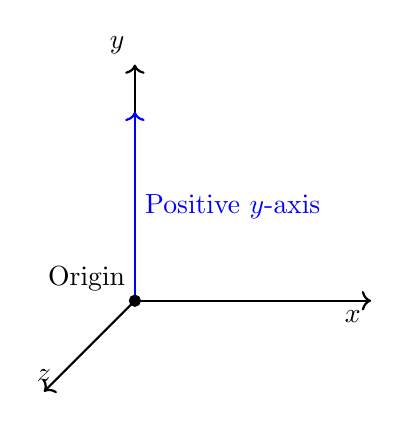
\begin{tikzpicture}[scale=2]

			% Draw the x, y, and z axes
			\draw[->, thick] (0,0,0) -- (1.5,0,0) node[anchor=north east] {$x$};
			\draw[->, thick] (0,0,0) -- (0,1.5,0) node[anchor=south east] {$y$}; % Positive y-axis
			\draw[->, thick] (0,0,0) -- (0,0,1.5) node[anchor=south] {$z$};

			% Positive y-axis with label
			\draw[->, thick, blue] (0,0,0) -- (0,1.2,0) node[midway,right] {Positive $y$-axis};

			% Draw a point at the origin
			\filldraw[black] (0,0,0) circle (1pt) node[anchor=south east] {Origin};

		\end{tikzpicture}
	\end{center}
}

\dfn{Standard Basis Vecotrs}{
	In an $n$-dimensional space $\mathbb{R}^n$, the standard basis vectors are a set of $n$ vectors where each vector has a 1 in one component and 0 in all other components. These vectors are denoted as $\mathbf{e}_i$ for $i = 1, 2, \dots, n$.

	The $i$-th standard basis vector in $\mathbb{R}^n$ is written as:

	\[
		\mathbf{e}_i =
		\begin{pmatrix}
			0                                       \\
			0                                       \\
			\vdots                                  \\
			1 \quad \text{(in the $i$-th position)} \\
			\vdots                                  \\
			0
		\end{pmatrix}
	\]

	For example, in $\mathbb{R}^3$ (three-dimensional space), the standard basis vectors are:

	\[
		\mathbf{e}_1 = \begin{pmatrix} 1 \\ 0 \\ 0 \end{pmatrix}, \quad
		\mathbf{e}_2 = \begin{pmatrix} 0 \\ 1 \\ 0 \end{pmatrix}, \quad
		\mathbf{e}_3 = \begin{pmatrix} 0 \\ 0 \\ 1 \end{pmatrix}.
	\]

	These vectors span the entire vector space $\mathbb{R}^n$, meaning any vector $\mathbf{v} \in \mathbb{R}^n$ can be written as a linear combination of the standard basis vectors:

	\[
		\mathbf{v} = v_1 \mathbf{e}_1 + v_2 \mathbf{e}_2 + \dots + v_n \mathbf{e}_n,
	\]

	where $v_1, v_2, \dots, v_n$ are the components of the vector $\mathbf{v}$.
}

\section{Operations}

\subsection{Dot Product}
\dfn{Dot (Scalar)Product Definitons}{
	The \textbf{scalar product} (or \textbf{dot product}) of two vectors \( \mathbf{a} \) and \( \mathbf{b} \) in \( \mathbb{R}^n \) is defined as:
	\[
		\mathbf{a} \cdot \mathbf{b} = a_1b_1 + a_2b_2 + \dots + a_nb_n
	\]
	In \( \mathbb{R}^3 \), for vectors \( \mathbf{a} = \begin{pmatrix} a_1 \\ a_2 \\ a_3 \end{pmatrix} \) and \( \mathbf{b} = \begin{pmatrix} b_1 \\ b_2 \\ b_3 \end{pmatrix} \), the dot product is:
	\[
		\mathbf{a} \cdot \mathbf{b} = a_1b_1 + a_2b_2 + a_3b_3
	\]
	The dot product can also be expressed in terms of the magnitudes of \( \mathbf{a} \) and \( \mathbf{b} \) and the angle \( \theta \) between them:
	\[
		\mathbf{a} \cdot \mathbf{b} = |\mathbf{a}| |\mathbf{b}| \cos \theta
	\]
	The dot product is a scalar quantity and is zero when the vectors are orthogonal (perpendicular).
	\\
	Useful to find the angle between the two vectors being dot produced together,

}

\thm{Dot Product Proof}{
	We are given the vectors $\vec{v}$ and $\vec{w}$, and we want to express the dot product in terms of their magnitudes and the angle between them.

	Start with the relationship:

	\[
		\vec{x} = \vec{v} - \vec{w}
	\]

	\begin{center}
		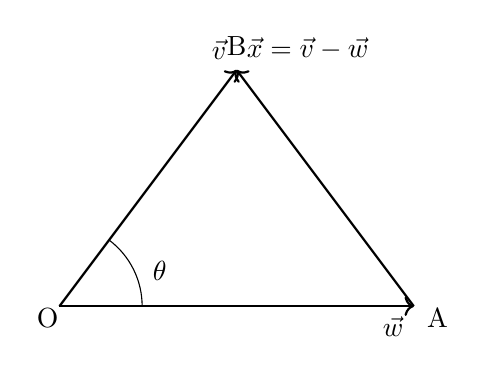
\begin{tikzpicture}[scale=1.5]
			% Draw vectors
			\draw[->, thick] (0,0) -- (3,0) node[anchor=north east] {$\vec{w}$};
			\draw[->, thick] (0,0) -- (1.5,2) node[anchor=south east] {$\vec{v}$};
			\draw[->, thick] (3,0) -- (1.5,2) node[anchor=south west] {$\vec{x} = \vec{v} - \vec{w}$};

			% Label the angle theta
			\draw (0.7,0) arc[start angle=0,end angle=53,radius=0.7];
			\node at (0.85,0.3) {$\theta$};

			% Draw point labels
			\node at (-0.1,-0.1) {O};
			\node at (3.2,-0.1) {A};
			\node at (1.5,2.2) {B};
		\end{tikzpicture}
	\end{center}

	The above diagram illustrates the vectors $\vec{v}$, $\vec{w}$, and their difference $\vec{x} = \vec{v} - \vec{w}$, forming a triangle. The angle $\theta$ is between $\vec{v}$ and $\vec{w}$.

	The magnitude squared of $\vec{x}$ is:

	\[
		|\vec{x}|^2 = |\vec{v}|^2 + |\vec{w}|^2 - 2|\vec{v}||\vec{w}|\cos\theta
	\]

	This is the expansion of the law of cosines.

	Now, from the equation:

	\[
		|\vec{x}|^2 = \sqrt[2]{\left( (v_x - w_x)^2 + (v_y - w_y)^2 \right)}^2
	\]

	We conclude:

	\[
		|\vec{x}|^2 = |\vec{v}|^2 + |\vec{w}|^2 - 2 (\vec{v} \cdot \vec{w})
	\]

	Thus, we can express the dot product $\vec{v} \cdot \vec{w}$ as:

	\[
		\vec{v} \cdot \vec{w} = |\vec{v}||\vec{w}|\cos\theta
	\]
}

\subsection{Applications}

\nt{
	The dot product of two vectors $\vec{v} \cdot \vec{w}$ can take different values, leading to various interpretations of the relationship between the vectors. Below is a table describing some key cases:

	\begin{center}
		\begin{tabular}{|c|c|c|}
			\hline
			\textbf{Dot Product Value}                    & \textbf{Interpretation}         & \textbf{Relationship Between Vectors}                                                         \\
			\hline
			$\vec{v} \cdot \vec{w} = 0$                   & $\cos\theta = 0$                & Vectors are \textbf{perpendicular} (orthogonal), $\theta = 90^\circ$                          \\
			\hline
			$\vec{v} \cdot \vec{w} > 0$                   & $0 < \theta < 90^\circ$         & Vectors form an \textbf{acute angle}, pointing in the same general direction                  \\
			\hline
			$\vec{v} \cdot \vec{w} < 0$                   & $90^\circ < \theta < 180^\circ$ & Vectors form an \textbf{obtuse angle}, pointing in opposite general directions                \\
			\hline
			$\vec{v} \cdot \vec{w} = |\vec{v}||\vec{w}|$  & $\cos\theta = 1$                & Vectors are \textbf{parallel} and point in the \textbf{same direction}, $\theta = 0^\circ$    \\
			\hline
			$\vec{v} \cdot \vec{w} = -|\vec{v}||\vec{w}|$ & $\cos\theta = -1$               & Vectors are \textbf{parallel} but point in \textbf{opposite directions}, $\theta = 180^\circ$ \\
			\hline
		\end{tabular}
	\end{center}
}

\dfn{Vector Product (Cross Product)}{
	The \textbf{vector product} (or \textbf{cross product}) of two vectors \( \mathbf{a} \) and \( \mathbf{b} \) in \( \mathbb{R}^3 \) is a vector \( \mathbf{c} \) that is perpendicular to both \( \mathbf{a} \) and \( \mathbf{b} \), and its magnitude is given by:
	\[
		|\mathbf{c}| = |\mathbf{a} \times \mathbf{b}| = |\mathbf{a}| |\mathbf{b}| \sin \theta
	\]
	where \( \theta \) is the angle between \( \mathbf{a} \) and \( \mathbf{b} \). The cross product is calculated as:
	\[
		\mathbf{a} \times \mathbf{b} = \begin{vmatrix}
			\hat{i} & \hat{j} & \hat{k} \\
			a_1     & a_2     & a_3     \\
			b_1     & b_2     & b_3
		\end{vmatrix} = (a_2b_3 - a_3b_2)\hat{i} - (a_1b_3 - a_3b_1)\hat{j} + (a_1b_2 - a_2b_1)\hat{k}
	\]
	The result of a cross product is a vector perpendicular to the plane formed by \( \mathbf{a} \) and \( \mathbf{b} \), with a direction given by the right-hand rule.
}

\dfn{Vector Projections} {
% Vector projection diagram

\begin{center}
	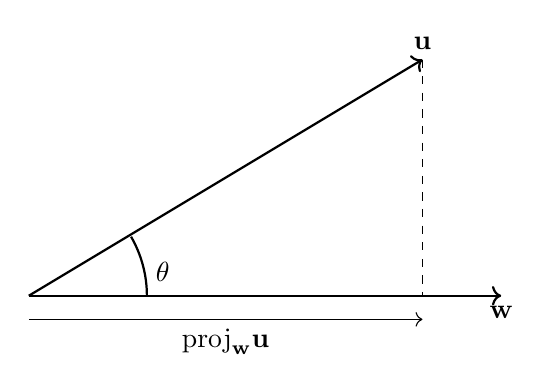
\begin{tikzpicture}
		% Draw vector w
		\draw[->, thick] (0,0) -- (6,0) node[anchor=north] {$\mathbf{w}$};

		% Draw vector u
		\draw[->, thick] (0,0) -- (5,3) node[anchor=south] {$\mathbf{u}$};

		% Projection line
		\draw[dashed] (5,3) -- (5,0) node[anchor=north] {};

		% Angle theta
		\draw[thick] (1.5,0) arc (0:30:1.5);
		\node at (1.7,0.3) {$\theta$};

		% Label projection of u on w
		\draw[->] (0,-0.3) -- (5,-0.3) node[midway,below] {$\text{proj}_{\mathbf{w}}\mathbf{u}$};
	\end{tikzpicture}
\end{center}

\[
	\text{scal}_{\mathbf{w}}\mathbf{u} = |\mathbf{u}| \cdot \cos\theta = \frac{\mathbf{w} \cdot \mathbf{u}}{|\mathbf{w}|}
\]

\[
	\text{proj}_{\mathbf{w}} \mathbf{u} = |\mathbf{u}| \cos \theta \left( \frac{\mathbf{w}}{|\mathbf{w}|} \right)
\]

\[
	\text{proj}_{\mathbf{w}} \mathbf{u} = \left( \frac{\mathbf{w} \cdot \mathbf{u}}{\mathbf{w} \cdot \mathbf{w}} \right) \mathbf{w}
\]
}

\section{Matrix Determinants}

\dfn{Matrix Representation}{
	A matrix is a collection of numbers arranged in a grid format, where each element is positioned based on its row and column. A general $m \times n$ matrix is written as:
	\[
		M =
		\begin{pmatrix}
			a_{11} & a_{12} & \cdots & a_{1n} \\
			a_{21} & a_{22} & \cdots & a_{2n} \\
			\vdots & \vdots & \ddots & \vdots \\
			a_{m1} & a_{m2} & \cdots & a_{mn} \\
		\end{pmatrix}
	\]
	For example, a $2 \times 2$ matrix is given by:
	\[
		M = \begin{pmatrix} a & b \\ c & d \end{pmatrix}
	\]
	A $3 \times 3$ matrix is:
	\[
		M = \begin{pmatrix} a & b & c \\ d & e & f \\ g & h & i \end{pmatrix}
	\]
	Matrices can be considered as a collection of vectors where each row or column can represent a vector.
}

\nt{\textbf{Vector Representation} \\
	A matrix can also be viewed as a collection of vectors. For instance, a $3 \times 3$ matrix can be interpreted as:
	\[
		M = \begin{pmatrix}
			\vec{v_1} = \langle a, b, c \rangle \\
			\vec{v_2} = \langle d, e, f \rangle \\
			\vec{v_3} = \langle g, h, i \rangle
		\end{pmatrix}
	\]
	where each row (or column) is treated as a vector in space.
}

\dfn{Determinant of a $2 \times 2$ Matrix}{
	The determinant of a $2 \times 2$ matrix is given by:
	\[
		\text{det}(M) = \det\begin{pmatrix} a & b \\ c & d \end{pmatrix} = ad - bc
	\]
	The determinant represents the signed area of the parallelogram formed by the vectors corresponding to the rows (or columns) of the matrix.


	\begin{center}
		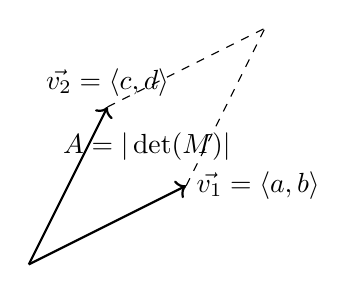
\begin{tikzpicture}
			% Define the vectors
			\draw[->, thick] (0,0) -- (2,1) node[right] {$\vec{v_1} = \langle a, b \rangle$};
			\draw[->, thick] (0,0) -- (1,2) node[above] {$\vec{v_2} = \langle c, d \rangle$};

			% Draw the parallelogram
			\draw[dashed] (2,1) -- (3,3);
			\draw[dashed] (1,2) -- (3,3);

			% Label the area
			\node at (1.5, 1.5) {$A = |\det(M)|$};
		\end{tikzpicture}
	\end{center}

}

\nt{\textbf{Geometric Interpretation} \\
	For a $2 \times 2$ matrix, the determinant represents the area $A$ of the parallelogram formed by the two vectors $\vec{v_1} = \langle a, b \rangle$ and $\vec{v_2} = \langle c, d \rangle$. The magnitude of the determinant gives the area of this parallelogram, and the sign of the determinant indicates the orientation (whether the vectors are ordered clockwise or counterclockwise).
}

\dfn{Determinant of a $3 \times 3$ Matrix}{
	The determinant of a $3 \times 3$ matrix is calculated as:
	\[
		\text{det}(M) = \det \begin{pmatrix}
			a & b & c \\
			d & e & f \\
			g & h & i
		\end{pmatrix}
		= a \det \begin{pmatrix} e & f \\ h & i \end{pmatrix}
		- b \det \begin{pmatrix} d & f \\ g & i \end{pmatrix}
		+ c \det \begin{pmatrix} d & e \\ g & h \end{pmatrix}
	\]
	The determinant represents the signed volume of the parallelepiped formed by the three vectors corresponding to the rows (or columns) of the matrix.
	\begin{center}
		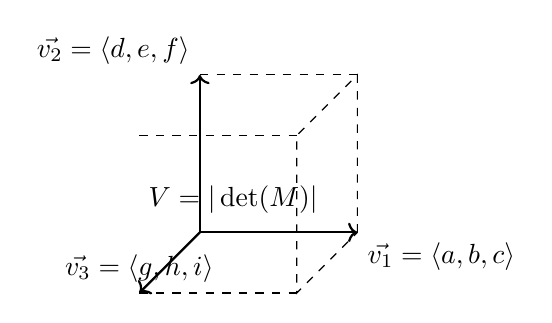
\begin{tikzpicture}
			% Define the 3D vectors
			\draw[->, thick] (0,0,0) -- (2,0,0) node[below right] {$\vec{v_1} = \langle a, b, c \rangle$};
			\draw[->, thick] (0,0,0) -- (0,2,0) node[above left] {$\vec{v_2} = \langle d, e, f \rangle$};
			\draw[->, thick] (0,0,0) -- (0,0,2) node[above] {$\vec{v_3} = \langle g, h, i \rangle$};

			% Draw the parallelepiped
			\draw[dashed] (2,0,0) -- (2,2,0) -- (2,2,2) -- (2,0,2) -- cycle;
			\draw[dashed] (0,2,0) -- (2,2,0);
			\draw[dashed] (0,0,2) -- (2,0,2);
			\draw[dashed] (0,2,2) -- (2,2,2);

			% Label the volume
			\node at (1,1,1.5) {$V = |\det(M)|$};
		\end{tikzpicture}
	\end{center}

}

\nt{\textbf{Geometric Interpretation for $3 \times 3$} \\
	In the $3 \times 3$ case, the determinant represents the volume $V$ of the parallelepiped formed by three vectors $\vec{v_1}, \vec{v_2}, \vec{v_3}$, and the sign indicates whether the orientation is right-handed or left-handed. The magnitude gives the volume.
}

\section{Matrix multiplication with 2D Vectors}

\dfn{Vector Matrix Multiplication}{

	\[
		M = \begin{pmatrix} a_{11} & a_{12} \\ a_{21} & a_{22} \end{pmatrix}, \quad
		V = \begin{pmatrix} V_1 \\ V_2 \end{pmatrix}
	\]

	\[
		\hat{\mathbf{j}}M = \langle a_{11}V_1 + a_{12}V_2, a_{21}V_1 + a_{22}V_2 \rangle
	\]

	Given:
	\[
		\hat{i} = \langle 1, 0 \rangle \quad \hat{j} = \langle 0, 1 \rangle
	\]

	We can compute:
	\[
		iM = \langle a_{11}, a_{12} \rangle = a_1
	\]
	\[
		jM = \langle a_{21}, a_{22} \rangle = a_2
	\]

	Where:
	\[
		\mathbf{V} = V_1 \hat{i} + V_2 \hat{j}
	\]
	\[
		\hat{\mathbf{V}}M = \left( V_1 \hat{i} + V_2 \hat{j} \right) M
	\]
	\[
		= V_1 \hat{i} M + V_2 \hat{j} M
	\]
	\[
		= V_1 \mathbf{a}_1 + V_2 \mathbf{a}_2
	\]

}

\nt{
	\centering
	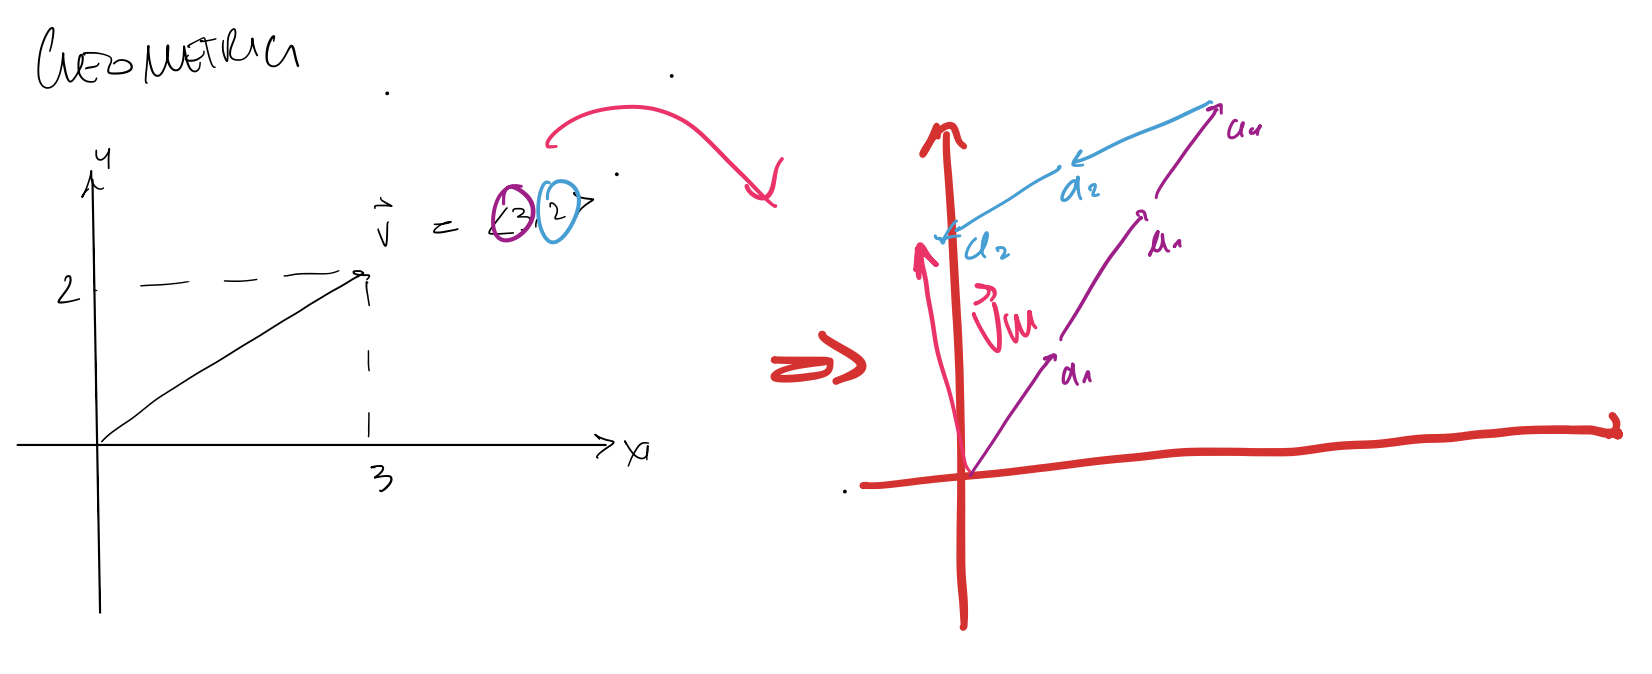
\includegraphics[width=0.5\textwidth]{graphicalvm.png} % Adjust the width as needed
	\par\vspace{1em} % Adds a small space after the image
}

\subsection{Effect on Area}

\dfn{$2D$}{
The original point \( (1,1) \) is transformed by the matrix \( M \). This transformation impacts the area and orientation as follows:

\[
	M = \begin{pmatrix} a_{11} & a_{12} \\ a_{21} & a_{22} \end{pmatrix}
\]

The area after transformation is given by the determinant of the matrix:

\[
	\text{Area} = \det(M)
\]
Where the determinant is calculated as:
\[
	\det(M) = a_{11}a_{22} - a_{12}a_{21}
\]

The determinant also determines the orientation:
\[
	\det(M) = \begin{cases}
		A  & \text{if } a_1 \text{ to } a_2 \text{ is counterclockwise} \\
		-A & \text{otherwise}
	\end{cases}
\]

In the example, the original vectors \( a_1 \) and \( a_2 \) form an area, and the determinant will tell us if the vectors are oriented in a clockwise or counterclockwise fashion.

If the determinant is negative, the orientation is clockwise, as illustrated:

\[
	\det \left( \begin{pmatrix} a_1 & a_2 \end{pmatrix} \right) < 0
\]

Thus, in this case, the transformation results in a clockwise orientation.
}

\section{Matrix multiplication with 3D Vectors}

\dfn{$3D$}{
	The matrix \( M \) for a 3D transformation is given as:

	\[
		M = \begin{pmatrix}
			a_{11} & a_{12} & a_{13} \\
			a_{21} & a_{22} & a_{23} \\
			a_{31} & a_{32} & a_{33}
		\end{pmatrix}
		\quad
		\text{where} \quad
		\vec{V} = \langle V_1, V_2, V_3 \rangle
	\]

	The transformation of vector \( \vec{V} \) under matrix \( M \) is:

	\[
		\hat{\vec{V}} M = \langle (a_{11} V_1 + a_{12} V_2 + a_{13} V_3), (a_{21} V_1 + a_{22} V_2 + a_{23} V_3), (a_{31} V_1 + a_{32} V_2 + a_{33} V_3) \rangle
	\]

	This can be written in terms of the basis vectors as:
	\[
		\left( V_1 \hat{i} + V_2 \hat{j} + V_3 \hat{k} \right) M = V_1 \vec{a}_1 + V_2 \vec{a}_2 + V_3 \vec{a}_3
	\]

}

\dfn{orientation and Volume}{
	- If the determinant of matrix \( M \) is negative, the system is **left-handed**, i.e.,
	\[
		\det(M) = -V
	\]
	- The determinant of the matrix \( M \) gives the **volume** of the parallelepiped spanned by the vectors \( a_1, a_2, a_3 \):

	\[
		\det(M) = \text{Volume}(V)
	\]

	The volume \( V \) is given by:
	\[
		V = \begin{cases}
			+V & \text{if } \vec{a}_1, \vec{a}_2, \vec{a}_3 \text{ are right-handed (RHS)} \\
			-V & \text{otherwise (left-handed)}
		\end{cases}
	\]
}

\section{Cross Product and Volumes}

\dfn{Cross Product and Volumes}{
	The volume of a parallelepiped defined by three vectors \( \vec{u}, \vec{v}, \vec{w} \) is given by:
	\[
		\text{V} = \vec{u} \cdot (\vec{v} \times \vec{w})
	\]
}

\subsection{Link to Matrix Determinants}

\dfn{Cross Product and Matrix Determinants}{
	\textbf{Since:}
	\[
		\vec{u} \cdot (\vec{v} \times \vec{w}) = \det \begin{pmatrix} \vec{u} & \vec{v} & \vec{w} \end{pmatrix}
	\]

	\[
		\det \begin{pmatrix}
			u_1 & u_2 & u_3 \\
			v_1 & v_2 & v_3 \\
			w_1 & w_2 & w_3
		\end{pmatrix}
		=
		u_1 \det \begin{pmatrix} v_2 & v_3 \\ w_2 & w_3 \end{pmatrix}
		- u_2 \det \begin{pmatrix} v_1 & v_3 \\ w_1 & w_3 \end{pmatrix}
		+ u_3 \det \begin{pmatrix} v_1 & v_2 \\ w_1 & w_2 \end{pmatrix}
	\]

	\[
		= \vec{u} \cdot
		\left(
		\hat{i} \begin{vmatrix} v_2 & v_3 \\ w_2 & w_3 \end{vmatrix}
		- \hat{j} \begin{vmatrix} v_1 & v_3 \\ w_1 & w_3 \end{vmatrix}
		+ \hat{k} \begin{vmatrix} v_1 & v_2 \\ w_1 & w_2 \end{vmatrix}
		\right)
	\]

	\[
		= \vec{u} \cdot \det \begin{pmatrix} \hat{i} & \hat{j} & \hat{k} \\ v_1 & v_2 & v_3 \\ w_1 & w_2 & w_3 \end{pmatrix}
	\]

	\[
		= \vec{u} \cdot (\vec{v} \times \vec{w})
	\]

	\textbf{Therefore:}

	\[
		\vec{v} \times \vec{w} = \det \begin{pmatrix} \hat{i} & \hat{j} & \hat{k} \\ v_1 & v_2 & v_3 \\ w_1 & w_2 & w_3 \end{pmatrix}
	\]
}

\section {Cross Product Polynomial Multiplication}

\dfn{Properties}{

	\[
		\hat{i} \times \hat{j} = \hat{k}, \quad \hat{j} \times \hat{k} = \hat{i}, \quad \hat{k} \times \hat{i} = \hat{j}
	\]

	\[
		\hat{j} \times \hat{i} = -\hat{k}, \quad \hat{i} \times \hat{i} = \hat{j} \times \hat{j} = \hat{k} \times \hat{k} = 0
	\]
}

\ex{Example: Cross Product}{
	Let \( \vec{v} = 2\hat{i} - \hat{j} - 3\hat{k} \) and \( \vec{w} = \hat{i} + \hat{j} + \hat{k} \). The cross product \( \vec{v} \times \vec{w} \) is computed as:

	\[
		\vec{v} \times \vec{w} = \left( 2\hat{i} - \hat{j} - 3\hat{k} \right) \times \left( \hat{i} + \hat{j} + \hat{k} \right)
	\]

	Expanding the cross product term by term:

	\[
		= 2\hat{i} \times \hat{i} + 2\hat{i} \times \hat{j} + 2\hat{i} \times \hat{k}
		- \hat{j} \times \hat{i} - \hat{j} \times \hat{j} - \hat{j} \times \hat{k}
		- 3\hat{k} \times \hat{i} - 3\hat{k} \times \hat{j} - 3\hat{k} \times \hat{k}
	\]

	Using the cross product identities:

	\[
		= 0 + 2\hat{k} + 2(-\hat{j})
		- (-\hat{k}) + 0 - \hat{i}
		- 3\hat{j} + 3\hat{i} + 0
	\]

	Combining like terms:

	\[
		= (3\hat{i} - \hat{i}) + (-2\hat{j} - 3\hat{j}) + (2\hat{k} + \hat{k})
	\]

	\[
		= 2\hat{i} - 5\hat{j} + 3\hat{k}
	\]

	Thus, the final result is:

	\[
		\vec{v} \times \vec{w} = 2\hat{i} - 5\hat{j} + 3\hat{k}
	\]
}

\section{Torque}

\dfn{Torque and Angular Momentum}{
	Continue with Torque
}


\section{Parametric Equations}

\dfn{Parametric Equations}{
	A parametric equation expresses a set of quantities as explicit functions of an independent parameter. In a two-dimensional case, a parametric equation for a curve can be represented as:
	\[
		\langle x,y  \rangle t = \langle f(t), g(t) \rangle
	\]
	and in three dimensions as:
	\[
		\langle x, y, z \rangle t = \langle f(t), g(t), h(t) \rangle
	\]
}

\nt{
	For example, consider the curve in the plane given by the equation \( y = f(x) = x^2 + 1 \). This describes a parabola in Cartesian coordinates.
}

\thm{Parametric unit circle in Cartesian coordinates}{
	A unit circle in parametric form can be represented as:
	\[
		x^2 + y^2 = 1
	\]
	which corresponds to the parametric equations:
	\[
		\langle x,y  \rangle t = \langle \cos(t), \sin(t) \rangle
	\]
}

\subsection{Examples}

\nt{
	The parametric equation:
	\[
		\langle x,y  \rangle t = \langle 4 \cos(t), 3 \sin(t) \rangle
	\]
	At specific values of \( t \), we can compute the points:
	\[
		t = 0 \implies \langle 4, 0 \rangle
	\]
	\[
		t = \frac{\pi}{2} \implies \langle 0, 3 \rangle
	\]
	\[
		t = \pi \implies \langle -4, 0 \rangle
	\]
	\[
		t = \frac{3\pi}{2} \implies \langle 0, -3 \rangle
	\]
}

\dfn{Parametric for a Helix}{
	\[
		\langle x(t), y(t), z(t) \rangle = \langle 4 \cos(t), 3 \sin(t), 0.1t \rangle
	\]
}

% The figure needs to be outside the definition environment
\begin{figure}[!htbp]
	\centering
	\vspace*{10pt}
	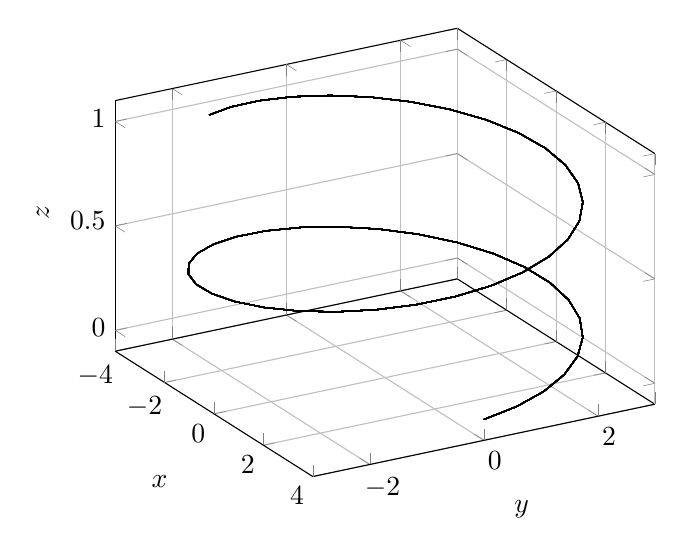
\begin{tikzpicture}
		\begin{axis}[mesh,
				samples=100,
				xlabel={$x$},
				ylabel={$y$},
				zlabel={$z$},
				view={60}{30},
				grid=both,
			]
			\addplot3 [
				domain=0:10,
				samples=50,
			]
			({4*cos(deg(x))}, {3*sin(deg(x))}, {0.1*x});
		\end{axis}
	\end{tikzpicture}
	\caption{3D plot of a parametric helix.}
	\label{fig:3dplot}
\end{figure}

\thm{Parametric Equation of a Line}{
	The parametric equation of a line can be expressed as:
	\[
		\langle x, y, z \rangle t = \mathbf{OP} + \mathbf{V}t
	\]
	Where:
	\begin{itemize}
		\item \( \mathbf{OP} = \langle x_0, y_0, z_0 \rangle \) is the position vector to the initial point \( P \),
		\item \( \mathbf{V} = \langle v_x, v_y, v_z \rangle \) is the direction vector of the line.
	\end{itemize}
}

\qs{3D Parametric Equation of a Line}{
	\begin{itemize}
		\item \( \mathbf{OP} = \langle 1, 2, 3 \rangle \) is the position vector to the initial point \( P \),
		\item \( \mathbf{V} = \langle 1, 1, 1 \rangle \) is the direction vector of the line.
	\end{itemize}
	Thus, the parametric equation of the line becomes:
	\[
		\langle x(t), y(t), z(t) \rangle = \langle 1, 2, 3 \rangle + t \langle 1, 1, 1 \rangle
	\]
	\[
		x(t) = 1 + t, \quad y(t) = 2 + t, \quad z(t) = 3 + t
	\]
	Or simply:
	\[
		\langle x, y, z \rangle t = \langle 1+t, 2+t, 3+t \rangle
	\]

}

\sol


% The figure for the parametric line
\begin{figure}[!htbp]
	\centering
	\vspace*{10pt}
	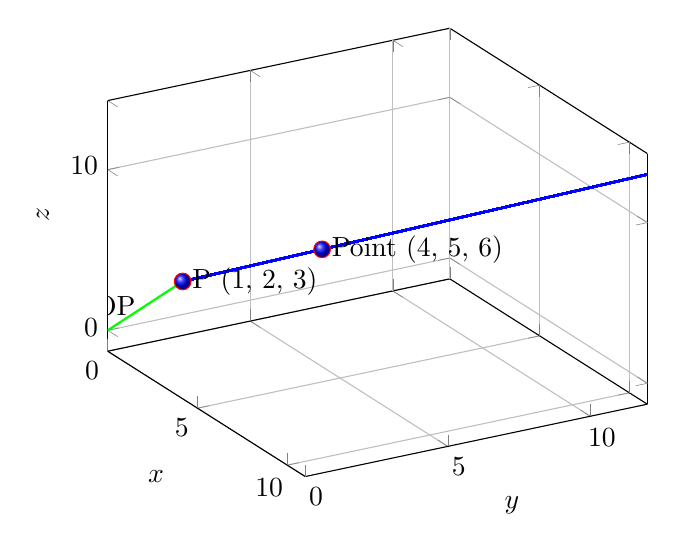
\begin{tikzpicture}
		\begin{axis}[mesh,
				samples=100,
				xlabel={$x$},
				ylabel={$y$},
				zlabel={$z$},
				view={60}{30},
				grid=both,
			]
			% Plot the parametric line
			\addplot3 [
				domain=0:10,
				samples=50,
				thick,
				color=blue,
			]
			({1 + x}, {2 + x}, {3 + x});

			% Mark the initial point OP = (1, 2, 3)
			\addplot3 [
				only marks,
				mark=ball,
				mark size=3pt,
				color=red,
			]
			coordinates {(1, 2, 3)};

			% Label the initial point
			\node at (axis cs:1, 2, 3) [anchor=west] {P (1, 2, 3)};

			% Plot the vector from the origin
			\addplot3 [
				-stealth,
				thick,
				color=green,
			]
			coordinates {(0, 0, 0) (1, 2, 3)};

			% Label the vector
			\node at (axis cs:0.5, 1, 1.5) [anchor=east] {OP};

			% Mark another point on the line for t = 3, (4, 5, 6)
			\addplot3 [
				only marks,
				mark=ball,
				mark size=3pt,
				color=red,
			]
			coordinates {(4, 5, 6)};

			% Label the point
			\node at (axis cs:4, 5, 6) [anchor=west] {Point (4, 5, 6)};
		\end{axis}
	\end{tikzpicture}
	\caption{3D plot of a parametric line with vector OP and points.}
	\label{fig:3dlineplot}
\end{figure}


\section{Distance from a Point to a Line}

\dfn{Parametric Equation of the Line}{
	The line is represented by:
	\[
		\mathbf{l} = \mathbf{OP} + t \mathbf{V}
	\]
	Where:
	\begin{itemize}
		\item \( \mathbf{OP} \) is the position vector of a point on the line,
		\item \( \mathbf{V} \) is the direction vector of the line.
	\end{itemize}
}

\thm{Distance from a Point to a Line}{
	The distance \( d \) from a point \( Q \) to the line \( l \) is given by:
	\[
		d = \frac{| \mathbf{V} \times \mathbf{PQ} |}{| \mathbf{V} |}
	\]
	Where:
	\begin{itemize}
		\item \( \mathbf{PQ} \) is the vector from point \( P \) on the line to the point \( Q \),
		\item \( \mathbf{V} \times \mathbf{PQ} \) is the cross product of the direction vector \( \mathbf{V} \) and the vector \( \mathbf{PQ} \).
	\end{itemize}
}

\subsection{Example}

\qs{Find the distance from the point \( Q = (3, 4, 0) \) to the line \( l \) given by the parametric equation}{
	\[
		\mathbf{l} = \langle t, 1, 2t \rangle = \langle 0, 1, 0 \rangle + t \langle 1, 0, 2 \rangle
	\]
	with point \( P = (0, 1, 0) \) and direction vector \( \mathbf{V} = \langle 1, 0, 2 \rangle \).
}

\sol
The vector \( \mathbf{PQ} \) from \( P = (0, 1, 0) \) to \( Q = (3, 4, 0) \) is:
\[
	\mathbf{PQ} = \langle 3, 4, 0 \rangle - \langle 0, 1, 0 \rangle = \langle 3, 3, 0 \rangle
\]
Now, we compute the cross product \( \mathbf{V} \times \mathbf{PQ} \):
\[
	\mathbf{V} \times \mathbf{PQ} = \begin{vmatrix}
		\hat{i} & \hat{j} & \hat{k} \\
		1       & 0       & 2       \\
		3       & 3       & 0       \\
	\end{vmatrix}
	= \hat{i}(0 - 6) - \hat{j}(0 - 6) + \hat{k}(3 - 0) = \langle -6, -6, 3 \rangle
\]
Next, calculate the magnitude of the cross product:
\[
	|\mathbf{V} \times \mathbf{PQ}| = \sqrt{(-6)^2 + (-6)^2 + 3^2} = \sqrt{36 + 36 + 9} = \sqrt{81} = 9
\]
The magnitude of the direction vector \( \mathbf{V} \) is:
\[
	|\mathbf{V}| = \sqrt{1^2 + 0^2 + 2^2} = \sqrt{1 + 4} = \sqrt{5}
\]
Finally, the distance \( d \) is:
\[
	d = \frac{9}{\sqrt{5}} = \frac{9\sqrt{5}}{5}
\]


\section{Intersection of Two Parametric Lines}

\dfn{Intersection of Parametric Lines}{
	To find the intersection point of two parametric lines, we need to equate their parametric equations and solve for the parameters.
}

\qs{Find the intersection of the lines \( l_1 \) and \( l_2 \) given by the parametric equations}{
	\[
		l_1 = \langle x, y \rangle (t) = \langle 0, 1 \rangle + t \langle 1, 0 \rangle
	\]
	\[
		l_2 = \langle 1, 1 \rangle + s \langle -2, 1 \rangle
	\]
}

\sol
Equating the two parametric equations:
\[
	\langle 0, 1 \rangle + t \langle 1, 0 \rangle = \langle 1, 1 \rangle + s \langle -2, 1 \rangle
\]
This gives the system of equations:
\[
	0 + t = 1 - 2s
\]
\[
	1 + 0 = 1 + s
\]

From the second equation, we find:
\[
	s = 0
\]

Substitute \( s = 0 \) into the first equation:
\[
	t = 1
\]

Thus, the lines intersect when \( t = 1 \) and \( s = 0 \).

The intersection point is:
\[
	\langle 0, 1 \rangle + 1 \cdot \langle 1, 0 \rangle = \langle 1, 1 \rangle
\]
Therefore, the lines intersect at \( (1, 1) \).

\section{Planes}

\dfn{Plane Equation}{
	Given a point \(P_0 = (x_0, y_0, z_0)\) on the plane and a normal vector \(\vec{n} = \langle a, b, c \rangle\), the equation of the plane can be expressed as:
	\[
		a(x - x_0) + b(y - y_0) + c(z - z_0) = 0
	\]
}

\nt{\textbf{Vector Form} \\
	Alternatively, the plane equation can also be derived using the dot product form:
	\[
		\overrightarrow{PQ} \cdot \vec{n} = 0
	\]
	Where \(P = (x_0, y_0, z_0)\) and \(Q = (x, y, z)\). This leads to the scalar equation of the plane.
}

\thm{Equation of a Plane}{
	If a plane passes through the point \(P_0 = (x_0, y_0, z_0)\) and has a normal vector \(\vec{n} = \langle a, b, c \rangle\), the equation of the plane is:
	\[
		a(x - x_0) + b(y - y_0) + c(z - z_0) = 0
	\]
}

\qs{Example}{
	Given the point \(P_0 = (1, -2, 3)\) and the normal vector \(\vec{n} = \langle -2, -4, -6 \rangle\), find the equation of the plane.
}

\sol
Using the plane equation \(a(x - x_0) + b(y - y_0) + c(z - z_0) = 0\), substitute \(a = -2\), \(b = -4\), \(c = -6\), and \(P_0 = (1, -2, 3)\):
\[
	-2(x - 1) - 4(y + 2) - 6(z - 3) = 0
\]
Expanding this equation:
\[
	-2x + 2 - 4y - 8 - 6z + 18 = 0
\]
Simplifying:
\[
	-2x - 4y - 6z + 12 = 0
\]
Or:
\[
	2x + 4y + 6z = 12
\]

\section{Vector Valued Functions}

\dfn{Parametric Curves}{
	A parametric curve is defined as:
	\[
		\vec{r}(t) = \langle x(t), y(t), z(t) \rangle = \langle f(t), h(t), g(t) \rangle
	\]
	where \(t\) is a real number as input, and the output is a vector.
}

\qs{Example}{
	Let \(\vec{r}(t) = \langle t^2, t+1, \sqrt{t - 2} \rangle\). Determine the domain of \(\vec{r}(t)\).
}

\sol
The domain of \(\vec{r}(t)\) is \(t \geq 2\).


\dfn{Limits of Vector Functions}{
	The limit of a vector function \(\vec{r}(t)\) as \(t \to a\) can be visualized geometrically as the vector approaching a point \(\vec{L}\). If the magnitude of the difference between \(\vec{L}\) and \(\vec{r}(t)\) approaches zero, we can define:
	\[
		\lim_{t \to a} \vec{r}(t) = \vec{L} \quad \text{if} \quad \lim_{t \to a} |\vec{L} - \vec{r}(t)| = 0
	\]
}


\begin{center}
	\begin{minipage}{0.32\textwidth}
		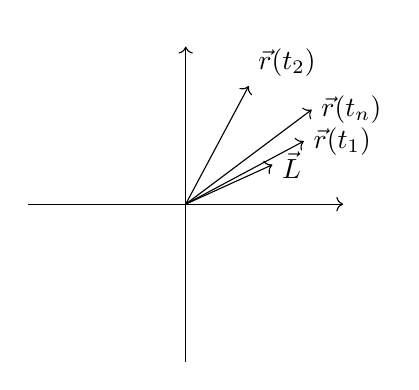
\begin{tikzpicture}
			% Axes
			\draw[->] (-2, 0) -- (2, 0) node[right] {};
			\draw[->] (0, -2) -- (0, 2) node[above] {};

			% Vectors from origin
			\draw[->] (0,0) -- (1.5, 0.8) node[right] {$\vec{r}(t_1)$};
			\draw[->] (0,0) -- (0.8, 1.5) node[above right] {$\vec{r}(t_2)$};
			\draw[->] (0,0) -- (1.6, 1.2) node[right] {$\vec{r}(t_n)$};
			\draw[->] (0,0) -- (1.1, 0.5) node[right] {$\vec{L}$};
		\end{tikzpicture}
	\end{minipage}%
	\begin{minipage}{0.32\textwidth}
		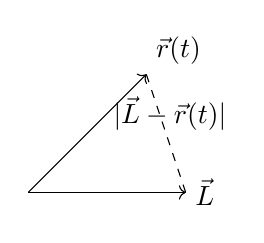
\begin{tikzpicture}
			% Triangle
			\draw[->] (0, 0) -- (2, 0) node[right] {$\vec{L}$};
			\draw[->] (0, 0) -- (1.5, 1.5) node[above right] {$\vec{r}(t)$};
			\draw[dashed] (1.5, 1.5) -- (2, 0);

			% Distance label
			\node at (1.8, 1.0) {$|\vec{L} - \vec{r}(t)|$};
		\end{tikzpicture}
	\end{minipage}
\end{center}


\nt{Component-wise Limits \\
	The limit of a vector function can be evaluated by taking the limit of each of its components:
	\[
		\lim_{t \to a} \vec{r}(t) = \langle \lim_{t \to a} x(t), \lim_{t \to a} y(t), \lim_{t \to a} z(t) \rangle
	\]
}

\qs{Example}{
	Consider the vector function \(\vec{r}(t) = \langle \frac{t^2 + 2t + 1}{t + 1}, t, t - 2 \rangle\), as \(t \to -1\).
}

\sol
The limits of each component as \(t \to -1\) are:

\[
	\lim_{t \to -1} \vec{r}(t) = \langle 0, -1, -3 \rangle
\]

\pagebreak

\section{Calculus and Vector Valued Functions}

\subsection{Derivative}

\thm{Derivative of vector functions}{
	Consider the vector-valued function in 3D:
	\[
		\vec{r}(t) = \langle f(t), g(t), h(t) \rangle
	\]
	where \( f(t), g(t) \), and \( h(t) \) are differentiable functions. The derivative of \( \vec{r}(t) \) is defined as:
	\[
		\vec{r}'(t) = \lim_{h \to 0} \frac{\vec{r}(t+h) - \vec{r}(t)}{h}
	\]

	Expanding \( \vec{r}(t+h) - \vec{r}(t) \):
	\[
		\vec{r}(t+h) - \vec{r}(t) = \langle f(t+h), g(t+h), h(t+h) \rangle - \langle f(t), g(t), h(t) \rangle
	\]
	This gives us:
	\[
		\vec{r}(t+h) - \vec{r}(t) = \langle f(t+h) - f(t), g(t+h) - g(t), h(t+h) - h(t) \rangle
	\]

	Thus, the derivative becomes:
	\[
		\vec{r}'(t) = \lim_{h \to 0} \left\langle \frac{f(t+h) - f(t)}{h}, \frac{g(t+h) - g(t)}{h}, \frac{h(t+h) - h(t)}{h} \right\rangle
	\]

	Since \( f(t), g(t) \), and \( h(t) \) are differentiable, we apply the definition of derivatives for each component:
	\[
		\vec{r}'(t) = \left\langle \lim_{h \to 0} \frac{f(t+h) - f(t)}{h}, \lim_{h \to 0} \frac{g(t+h) - g(t)}{h}, \lim_{h \to 0} \frac{h(t+h) - h(t)}{h} \right\rangle
	\]
	\[
		\vec{r}'(t) = \langle f'(t), g'(t), h'(t) \rangle
	\]

	Therefore, the derivative of the vector-valued function \( \vec{r}(t) \) in 3D is:
	\[
		\boxed{\vec{r}'(t) = \langle f'(t), g'(t), h'(t) \rangle}
	\]
}

\dfn{Vector Representation}{

	Let \( \vec{r}(t) \) be a vector-valued function that describes the position of a particle over time \( t \):
	\[
		\vec{r}(t) = \langle x(t), y(t), z(t) \rangle
	\]
	where \( x(t), y(t), z(t) \) are differentiable functions. The following terms describe important properties of the function:



	\begin{enumerate}
		\item \textbf{Position} at time \( t \): \( \vec{r}(t) \)
		\item \textbf{Velocity} (tangent vector) \( \vec{r}'(t) = \langle x'(t), y'(t), z'(t) \rangle \)
		\item \textbf{Speed} \( |\vec{r}'(t)| \), the magnitude of the velocity.
		\item \textbf{Acceleration} \( \vec{r}''(t) = \langle x''(t), y''(t), z''(t) \rangle \)

	\end{enumerate}
}

\dfn{Unit Tangent Vector}{

	The unit tangent vector is given by:
	\[
		\hat{T}(t) = \frac{\vec{r}'(t)}{|\vec{r}'(t)|}
	\]
	This is the unit vector in the direction of the velocity vector \( \vec{r}'(t) \), which represents the direction of motion.
}

\qs{Example}{
	Consider the following vector-valued function:
	\[
		\vec{r}(t) = \langle 1 + t^2, 2 + t^2, 3 + t^2 \rangle
	\]
	Taking the derivative:
	\[
		\vec{r}'(t) = \langle 2t, 2t, 2t \rangle
	\]
	This describes a line with a constant acceleration:
	\[
		\vec{r}''(t) = \langle 2, 2, 2 \rangle
	\]
}

\begin{tikzpicture}
	% The curve of position
	\draw[thick] (0,0) to[out=70,in=180] (4,4) to[out=0,in=160] (8,1);

	% Time labels
	\node at (0, 0) [below] {$t = 0$};
	\node at (4, 4) [above] {$t = 1$};
	\node at (8, 1) [right] {$t = 3$};

	% Velocity arrow at t=1
	\draw[->, magenta, thick] (4, 4) -- (6.5, 4) node[above right] {$\vec{r}'(t)$};

	% Acceleration arrow at t=3
	\draw[->, blue, thick] (8, 1) -- (9.5, 1.5) node[above] {$\vec{r}''(t)$};

	% Labels for position, velocity, acceleration
	\node at (3, 2) [green] {$\vec{r}(t)$};
	\node at (6, 5) [magenta] {Velocity $\vec{r}'(t)$};
	\node at (8.5, 0.5) [blue] {Acceleration $\vec{r}''(t)$};
\end{tikzpicture}

\dfn{Derivatives of Parametric Curves in terms of $t$}{

	Given a parametric curve defined by:
	\[
		x = f(t), \quad y = g(t)
	\]
	where \(t\) is the parameter, we want to find the derivative \(\frac{dy}{dx}\), which represents the slope of the tangent to the curve at any point \(t\).

	\textbf{Step 1: Finding the Derivatives of \(x\) and \(y\) with respect to \(t\)}
	To find \(\frac{dy}{dx}\), we need to find both \(\frac{dx}{dt}\) and \(\frac{dy}{dt}\). These are given by:
	\[
		\frac{dx}{dt} = f'(t), \quad \frac{dy}{dt} = g'(t)
	\]

	\textbf{Step 2: Using the Chain Rule}
	The derivative \(\frac{dy}{dx}\) can be found by using the chain rule as follows:
	\[
		\frac{dy}{dx} = \frac{\frac{dy}{dt}}{\frac{dx}{dt}}
	\]
	Substituting the expressions for \(\frac{dx}{dt}\) and \(\frac{dy}{dt}\), we obtain:
	\[
		\frac{dy}{dx} = \frac{g'(t)}{f'(t)}
	\]

	\textbf{Step 3: Simplifying the Result}
	The expression \(\frac{dy}{dx}\) provides the slope of the curve at any point \(t\) in terms of the parameter.
}

\ex{Consider the parametric equations:}{

	\[
		x = 6 \sin t, \quad y = 6 \cos t
	\]

	To find \(\frac{dy}{dx}\), we calculate the derivatives with respect to \(t\):
	\[
		\frac{dx}{dt} = 6 \cos t, \quad \frac{dy}{dt} = -6 \sin t
	\]

	Then, we apply the formula:
	\[
		\frac{dy}{dx} = \frac{\frac{dy}{dt}}{\frac{dx}{dt}} = \frac{-6 \sin t}{6 \cos t}
	\]

	Simplifying the expression:
	\[
		\frac{dy}{dx} = -\tan t
	\]

	Therefore, the slope of the tangent line to the parametric curve at any point \(t\) is:
	\[
		\frac{dy}{dx} = -\tan t
	\]
}

\dfn{Chain Rule Derivation}{
	\[
		\frac{dy}{dt} = \frac{dy}{du} \cdot \frac{dx}{dt} \quad \Rightarrow \quad \frac{dy}{dx} = \frac{\frac{dy}{dt}}{\frac{dx}{dt}}
		\quad \Rightarrow \quad \frac{dy}{dx} = \frac{du}{dt}
	\]
}

\qs{Example}{
	Slope of
	\[
		\vec{r}(t) = \langle \cos(t), \sin(t) \rangle
	\]

	At \( t = \frac{\pi}{3} \):

}

\sol

\[
	\cos\left(\frac{\pi}{3}\right) = \frac{1}{2}, \quad \sin\left(\frac{\pi}{3}\right) = \frac{\sqrt{3}}{2}
\]


\[
	\vec{r}'(t) = \langle -\sin(t), \cos(t) \rangle
\]


At \( t = \frac{\pi}{3} \):

\[
	\vec{r}'\left(\frac{\pi}{3}\right) = \langle -\frac{\sqrt{3}}{2}, \frac{1}{2} \rangle
\]

Slope Calculation
\[
	\text{slope} = \frac{\frac{-1}{2}}{\frac{-\sqrt{3}}{2}} = \frac{1}{\sqrt{3}} = \frac{\sqrt{3}}{3}
\]

Vector Notation
\[
	\vec{r}'(t) = \langle -\sin(t), \cos(t) \rangle \quad \text{so} \quad \vec{r}'\left(\frac{\pi}{3}\right) = \langle -\frac{\sqrt{3}}{2}, \frac{1}{2} \rangle
\]

\subsection{Chain Rule}

\dfn{Chain Rule for VV}{

	Let $g : \mathbb{R} \to \mathbb{R}$ and $\vec{r}(t)$ be a vector function. The derivative of the composition of functions is:

	\[
		\frac{d}{dt}[g(\vec{r}(t))] = g'(\vec{r}(t)) \cdot \vec{r}'(t)
	\]

	where $g'(\vec{r}(t))$ is the derivative of $g$ with respect to the vector function $\vec{r}(t)$ and $\vec{r}'(t)$ is the derivative of the vector function $\vec{r}(t)$ with respect to $t$. This rule is useful for differentiating scalar functions composed with vector-valued functions.

}

\qs{Example}{

\[
	\vec{r}(t) = \langle \cos^2 t, -3t + \cos^3 t \rangle = \dot{\vec{r}}(g(t))
\]
\[
	y = \cos t, \quad \vec{r} = \langle t^2, -3t, 3t^3 \rangle
\]
\[
	g' = -\sin t, \quad \dot{\vec{r}} = \langle 2t, 3t^2 \rangle
\]

Thus, the derivative is:

\[
\vec{s}(t) = \frac{d}{dt} \left( g(y(t)) \vec{r}(g(t)) \right) = g'(t) \cdot \dot{\vec{r}}(g(t))
\]

\[
= -\sin t \cdot \langle 2\cos t, 3\cos^2 t \rangle
\]

}

\subsection{Product Rule}

\dfn{Product rule for VV}{

	Let $g(t): \mathbb{R} \to \mathbb{R}$, $\vec{r}(t): \mathbb{R} \to \mathbb{R}^n$, and $\vec{s}(t): \mathbb{R} \to \mathbb{R}^n$ be vector functions. Then, the product rule is:

	\[
		\frac{d}{dt} \left( g(t) \vec{r}(t) \right) = g'(t) \vec{r}(t) + g(t) \dot{\vec{r}}(t)
	\]

	For vector dot products:

	\[
		\frac{d}{dt} \left( \vec{r}(t) \cdot \vec{s}(t) \right) = \vec{r}'(t) \cdot \vec{s}(t) + \vec{r}(t) \cdot \vec{s}'(t)
	\]

	For vector cross products:

	\[
		\frac{d}{dt} \left( \vec{r}(t) \times \vec{s}(t) \right) = \vec{r}'(t) \times \vec{s}(t) + \vec{r}(t) \times \vec{s}'(t)
	\]

}

\subsection{Integrals}

\dfn{Integral of Vector-Valued Functions}{

Let $\vec{r}(t): [a,b] \to \mathbb{R}^n$ be a continuous vector-valued function. The definite integral of $\vec{r}(t)$ over the interval $[a,b]$ is defined as:

\[
	\int_a^b \vec{r}(t) \, dt = \langle \int_a^b r_1(t) \, dt, \int_a^b r_2(t) \, dt, \dots, \int_a^b r_n(t) \, dt \rangle
\]

where $\vec{r}(t) = \langle r_1(t), r_2(t), \dots, r_n(t) \rangle$. This means that the integral of a vector-valued function is the vector whose components are the integrals of the respective component functions.

For example, if $\vec{r}(t) = \langle f(t), g(t), h(t) \rangle$, then:

\[
	\int_a^b \vec{r}(t) \, dt = \langle \int_a^b f(t) \, dt, \int_a^b g(t) \, dt, \int_a^b h(t) \, dt \rangle
\]

This can be extended to cases where $\vec{r}(t)$ represents the position of a particle over time, and the integral represents the net displacement of the particle over the interval $[a,b]$.

}

\qs{Find the integral of the vector-valued function}{Calculate the integral of the vector-valued function \(\vec{r}(t) = \langle t^2, \sin t, e^t \rangle\) over the interval \(t \in [0, 1]\).}

\sol

The vector-valued function is given as:

\[
	\vec{r}(t) = \langle t^2, \sin t, e^t \rangle
\]

We can integrate each component of the vector separately over the interval \([0, 1]\):

\[
	\int_0^1 \vec{r}(t) \, dt = \langle \int_0^1 t^2 \, dt, \int_0^1 \sin t \, dt, \int_0^1 e^t \, dt \rangle
\]

Now, solving each integral:

1. For \(\int_0^1 t^2 \, dt\):

\[
	\int_0^1 t^2 \, dt = \left[ \frac{t^3}{3} \right]_0^1 = \frac{1^3}{3} - \frac{0^3}{3} = \frac{1}{3}
\]

2. For \(\int_0^1 \sin t \, dt\):

\[
	\int_0^1 \sin t \, dt = \left[ -\cos t \right]_0^1 = -\cos(1) + \cos(0) = 1 - \cos(1)
\]

3. For \(\int_0^1 e^t \, dt\):

\[
	\int_0^1 e^t \, dt = \left[ e^t \right]_0^1 = e^1 - e^0 = e - 1
\]

Thus, the result of the integral is:

\[
	\int_0^1 \vec{r}(t) \, dt = \langle \frac{1}{3}, 1 - \cos(1), e - 1 \rangle
\]

\qs{Find the position vector of a ball in 3D space}{A ball is thrown from the origin with an initial velocity vector \(\vec{v}(0) = \langle 1, 3, 5 \rangle\) m/s, and experiences a constant acceleration vector \(\vec{a}(t) = \langle 0, 0, -10 \rangle\) m/s\(^2\). Find the position vector \(\vec{r}(t)\) of the ball at any time \(t\).}

\sol

The velocity vector \(\vec{v}(t)\) is found by integrating the acceleration vector \(\vec{a}(t)\):

\[
	\vec{v}(t) = \int_0^t \vec{a}(s) \, ds + \vec{v}(0)
\]

Given that \(\vec{a}(t) = \langle 0, 0, -10 \rangle\), we integrate each component:

\[
	\vec{v}(t) = \int_0^t \langle 0, 0, -10 \rangle \, ds + \langle 1, 3, 5 \rangle
\]
\[
	= \langle 0, 0, -10t \rangle + \langle 1, 3, 5 \rangle
\]
\[
	\vec{v}(t) = \langle 1, 3, 5 - 10t \rangle
\]

Now, to find the position vector \(\vec{r}(t)\), we integrate the velocity vector \(\vec{v}(t)\):

\[
	\vec{r}(t) = \int_0^t \vec{v}(s) \, ds
\]
\[
	= \int_0^t \langle 1, 3, 5 - 10s \rangle \, ds
\]

Integrating each component:

1. For the first component:
\[
	\int_0^t 1 \, ds = t
\]

2. For the second component:
\[
	\int_0^t 3 \, ds = 3t
\]

3. For the third component:
\[
	\int_0^t (5 - 10s) \, ds = \left[ 5s - 5s^2 \right]_0^t = 5t - 5t^2
\]

Thus, the position vector is:

\[
	\vec{r}(t) = \langle t, 3t, 5t - 5t^2 \rangle
\]

\pagebreak

\section{Arc Length}

The arc length of a smooth curve given by a vector-valued function can be calculated using an integral. Let the position vector of a curve be represented as:
\[
	\vec{r}(t) = \langle f(t), g(t), h(t) \rangle,
\]
where \(t\) is the parameter over some interval \([a, b]\).

\dfn{Arc Length Formula}{
	The arc length \(L\) of the curve \(\vec{r}(t)\) over the interval \([a, b]\) is given by:
	\[
		L = \int_a^b \left| \vec{r}'(t) \right| \, dt,
	\]
	where \(\vec{r}'(t)\) is the derivative of the position vector, representing the velocity vector of the curve.

	To find \(\left| \vec{r}'(t) \right|\), we use the following:
	\[
		\left| \vec{r}'(t) \right| = \sqrt{\left( f'(t) \right)^2 + \left( g'(t) \right)^2 + \left( h'(t) \right)^2}.
	\]

	Therefore, the arc length formula can be explicitly written as:
	\[
		L = \int_a^b \sqrt{\left( f'(t) \right)^2 + \left( g'(t) \right)^2 + \left( h'(t) \right)^2} \, dt.
	\]
}

\qs{Example: Eagle Spiraling}{
	Consider an example where an eagle is spiraling in space, and its position at time \(t\) (in minutes) is given by:
	\[
		\vec{r}(t) = \langle 250 \cos(t), 250 \sin(t), 100t \rangle \quad \text{(in feet)}.
	\]
}

\sol

To find the velocity vector, we differentiate each component of \(\vec{r}(t)\):
\[
	\vec{r}'(t) = \langle -250 \sin(t), 250 \cos(t), 100 \rangle \quad \text{(in feet per minute)}.
\]

The magnitude of the velocity vector \(\left| \vec{r}'(t) \right|\) is:
\[
	\left| \vec{r}'(t) \right| = \sqrt{(-250 \sin(t))^2 + (250 \cos(t))^2 + (100)^2}.
\]
Simplifying, we obtain:
\[
	\left| \vec{r}'(t) \right| = \sqrt{250^2 \sin^2(t) + 250^2 \cos^2(t) + 100^2}.
\]

Using the Pythagorean identity \(\sin^2(t) + \cos^2(t) = 1\), we find:
\[
	\left| \vec{r}'(t) \right| = \sqrt{250^2 + 100^2} = \sqrt{62500 + 10000} = \sqrt{72500} \approx 269.3 \quad \text{(feet per minute)}.
\]

Therefore, the speed of the eagle is approximately \(269.3\) feet per minute.

\qs{Calculating Distance Over Time}{Find the total distance over 10 minutes}

\sol

To find the total distance traveled by the eagle over a period of 10 minutes, we compute the arc length:
\[
	\text{Distance} = \int_0^{10} \left| \vec{r}'(t) \right| \, dt = \int_0^{10} 269.3 \, dt.
\]

Evaluating the integral:
\[
	\text{Distance} = 269.3 \cdot (10 - 0) = 2693 \text{ feet}.
\]

Thus, over 10 minutes, the eagle travels approximately 2693 feet.

\dfn{Arc Length Function}{
	The arc length function, denoted by \(S(t)\), is defined as:
	\[
		S(t) = \text{distance traveled along the curve from } t = a.
	\]
	It is given by the integral:
	\[
		S(t) = \int_a^t \left| \vec{r}'(s) \right| \, ds.
	\]
	This function essentially converts the vector quantity \(\vec{r}(t)\) into a 1-dimensional scalar that measures the total distance traveled without considering direction.

	The arc length function \(S(t)\) effectively flattens the vector \(\vec{r}(t)\) into a scalar by integrating the magnitude of the velocity vector \(\vec{r}'(s)\) over the interval \([a, t]\).
}

\ex{Application: Reparametrization by Arc Length}{
One common use of the arc length function is to reparametrize the curve so that it is traveled at unit speed.

Given the inverse function of \(S(t)\), denoted as \(S^{-1}(t)\), we wish to compare:
\[
	\vec{r}\left( S^{-1}(t) \right) \quad \text{with} \quad \vec{r}(t).
\]


If \(S(t)\) is given by:
\[
	S(t) = \int_a^t \left| \vec{r}'(p) \right| \, dp,
\]
then \(S'(t) = \left| \vec{r}'(t) \right|\).

To differentiate \(\vec{r}(S^{-1}(t))\), we use the chain rule:
\[
	\frac{d}{dt} \vec{r}(S^{-1}(t)) = \frac{1}{S'(S^{-1}(t))} \vec{r}'(S^{-1}(t)).
\]

Since \(S'(S^{-1}(t)) = \left| \vec{r}'(S^{-1}(t)) \right|\), we have:
\[
	\frac{d}{dt} \vec{r}(S^{-1}(t)) = \frac{\vec{r}'(S^{-1}(t))}{\left| \vec{r}'(S^{-1}(t)) \right|}.
\]
This shows that the derivative of \(\vec{r}(S^{-1}(t))\) is a unit vector, implying that \(\vec{r}(S^{-1}(t))\) describes the same curve as \(\vec{r}(t)\), but at unit speed.

By reparametrizing the curve with respect to arc length, we achieve a uniform traversal of the curve at constant unit speed. The transformation \(\vec{r}(S^{-1}(t))\) provides a way to describe the geometry of the curve without the influence of varying speed.

}

\qs{Worked Example}{
Consider the position of an eagle as it spirals upward over time. The position vector \(\vec{r}(t)\) is given by:
\[
	\vec{r}(t) = \langle 250 \cos(t), 250 \sin(t), 100t \rangle \quad \text{(in feet)},
\]
where \(t\) is in minutes.

\subsection*{Step 1: Find the Speed of the Eagle}
The velocity vector is obtained by differentiating the position vector:
\[
	\vec{r}'(t) = \langle -250 \sin(t), 250 \cos(t), 100 \rangle.
\]

The speed is the magnitude of the velocity vector:
\[
	\left| \vec{r}'(t) \right| = \sqrt{(-250 \sin(t))^2 + (250 \cos(t))^2 + 100^2} = \sqrt{62500 + 10000} = 269.3 \quad \text{(feet per minute)}.
\]

\subsection*{Step 2: Arc Length Function \(S(t)\)}
To find the arc length function \(S(t)\), which represents the distance traveled along the curve from \(t = 0\) to \(t = t\):
\[
	S(t) = \int_0^t \left| \vec{r}'(p) \right| \, dp.
\]
Since the speed is constant:
\[
	S(t) = \int_0^t 269.3 \, dp = 269.3 t.
\]

Thus, at time \(t\), the eagle has traveled \(269.3 t\) feet.

\subsection*{Step 3: Reparametrize by Arc Length}
The inverse of the arc length function \(S(t)\), denoted as \(S^{-1}(t)\), is given by:
\[
	S^{-1}(t) = \frac{t}{269.3}.
\]

Now, to reparametrize the curve by arc length, we substitute \(S^{-1}(t)\) into the original position vector \(\vec{r}(t)\):
\[
\vec{r}(S^{-1}(t)) = \left\langle 250 \cos\left( \frac{t}{269.3} \right), 250 \sin\left( \frac{t}{269.3} \right), 100 \frac{t}{269.3} \right\rangle.
\]

\subsection*{Interpretation}
This reparametrization gives the position of the eagle as a function of the distance traveled (in feet), rather than as a function of time. It provides a way to describe the motion of the eagle along the curve such that the eagle is moving at a constant speed of 1 foot per unit of time.

}

\section{Curvature of a Vector-Valued Function}
Curvature is a measure of the "sharpness" or "bendiness" of a curve. For a smooth curve given by a vector-valued function \(\vec{r}(t)\), the curvature at a point is related to how quickly the direction of the curve is changing.

\subsection{Osculating Circle}
The concept of curvature is closely tied to the idea of an \textbf{osculating circle}. At any point on the curve, the osculating circle is the circle that best approximates the curve's curvature at that point. This circle:
- Has the same tangent as the curve \(\vec{r}(t)\) at the point \(\vec{r}(t_0)\).
- Its radius is a measure of the "tightness" of the curve's bend at that point.

The radius of the osculating circle is denoted as:
\[
	R(t),
\]
where \(R(t)\) is the radius of curvature of the curve at time \(t\).

\subsection{Curvature \(\kappa(t)\)}
The curvature \(\kappa(t)\) of the curve \(\vec{r}(t)\) at the point \(\vec{r}(t_0)\) is defined as the reciprocal of the radius of the osculating circle:
\[
	\kappa(t) = \frac{1}{R(t)}.
\]
A smaller radius \(R(t)\) indicates a tighter bend and thus a larger curvature \(\kappa(t)\), whereas a larger radius corresponds to a gentler curve and smaller curvature.

The osculating circle provides a geometric interpretation of curvature, serving as the best circular approximation to the curve at any given point. The curvature \(\kappa(t)\) quantifies how sharply the curve bends at that point, with the relationship:
\[
	\kappa(t) = \frac{1}{R(t)}.
\]

\dfn{Osculating Circle of a Straight Line}{

	A straight line is a curve with no curvature. Thus, the curvature \(\kappa(t)\) of a straight line is zero at all points. To understand why, consider the definition of the osculating circle.


	For any curve \(\vec{r}(t)\), the osculating circle at a point \(\vec{r}(t_0)\) is defined as the circle that "best fits" the curve at that point. Mathematically, this means:
	\[
		\kappa(t) = \lim_{\Delta t \to 0} \frac{\text{change in angle}}{\text{arc length}},
	\]
	where \(\kappa(t)\) is the curvature of the curve. However, for a straight line, the change in angle is always zero, so:
	\[
		\kappa(t) = 0.
	\]

	Since curvature is the reciprocal of the radius of the osculating circle \(R(t)\), a zero curvature implies an infinite radius:
	\[
		R(t) = \frac{1}{\kappa(t)} \to \infty.
	\]
	Therefore, the osculating circle of a straight line is effectively a circle with infinite radius, meaning it is "flattened" into a straight line.

}

\subsection*{Diagram}
Below is a diagram to illustrate the concept of the osculating circle of a straight line:

\begin{center}
	\begin{tikzpicture}[scale=1.2]
		% Draw the straight line
		\draw[thick] (-3, 0) -- (3, 0) node[right] {\(\vec{r}(t)\)};

		% Draw the tangent vector at the point
		\draw[->, thick] (0, 0) -- (1, 0) node[above] {Tangent};

		% Mark a point on the line
		\filldraw (0, 0) circle (2pt) node[below] {\(\vec{r}(t_0)\)};

		% Draw the large osculating circle (only a visible arc to suggest a large radius)
		\draw[dashed] (5, 0) arc[start angle=0, end angle=180, radius=5];

		% Label the osculating circle
		\node at (0, 3.2) {Osculating circle (large radius)};
	\end{tikzpicture}
\end{center}

The dashed arc represents the osculating circle with an infinitely large radius, approximating the straight line at \(\vec{r}(t_0)\).

To approach the concept of osculating circles for vector-valued functions, we break down the analysis into four key points:

\subsection*{1. Tangent Vector at \(t_0\)}
The tangent vector to the curve at time \(t_0\) is given by:
\[
	\vec{T}(t) = \frac{\vec{r}'(t)}{\left| \vec{r}'(t) \right|}.
\]
This vector is the unit tangent vector at any point on the curve.

\subsection*{2. If \(\vec{r}(t)\) Describes a Circle}
Suppose that \(\vec{r}(t)\) describes a circular path. In this case:
\begin{itemize}
	\item The vector \(\vec{r}(t)\) is always parallel to the radius of the circle.
	\item The velocity vector \(\vec{r}'(t)\) is also perpendicular to \(\vec{r}(t)\).
\end{itemize}

\begin{center}
	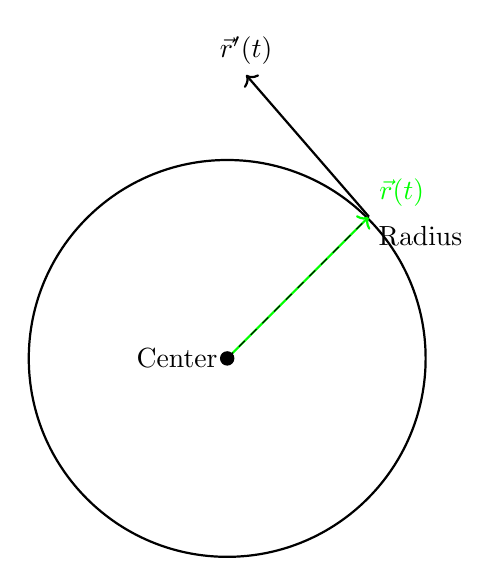
\begin{tikzpicture}[scale=1.2]
		% Draw the circle
		\draw[thick] (0,0) circle (2.1);

		% Draw the position vector
		\draw[->, thick, green] (0,0) -- (1.5,1.5) node[above right] {\(\vec{r}(t)\)};

		% Draw the radius (position vector)
		\draw[dashed] (0,0) -- (1.5,1.5) node[below right] {Radius};

		% Draw the tangent vector
		\draw[->, thick] (1.5,1.5) -- (0.2, 3) node[above] {\(\vec{r}'(t)\)};

		% Mark the center of the circle
		\filldraw (0,0) circle (2pt) node[left] {Center};
	\end{tikzpicture}
\end{center}

\subsection*{3. Acceleration Vector \(\vec{a}(t)\)}
For a circular path, the acceleration vector \(\vec{a}(t)\) points toward the center of the circle. Hence,
\[
	\vec{a}(t) \text{ is opposite to } \vec{r}(t) \text{ and directed towards the center}.
\]
This implies:
\[
	\vec{a}(t) \perp \vec{r}'(t), \quad \vec{a}(t) \perp \vec{T}(t).
\]

\subsection*{4. Constant Speed and Perpendicularity}
Suppose that \(\vec{r}(t)\) describes a curve with constant speed:
\[
	\left| \vec{r}'(t) \right| = C, \quad C \in \mathbb{R}.
\]

For both 2D and 3D, the curve will either be a circle or a sphere with a fixed radius. The velocity and acceleration vectors, \(\vec{r}'(t)\) and \(\vec{a}(t)\), maintain a perpendicular relationship:
\[
	\vec{r}(t) \cdot \vec{v}(t) = 0.
\]

\begin{center}
	\begin{minipage}{0.45\textwidth}
		\centering
		\subsection*{2D Circle}
		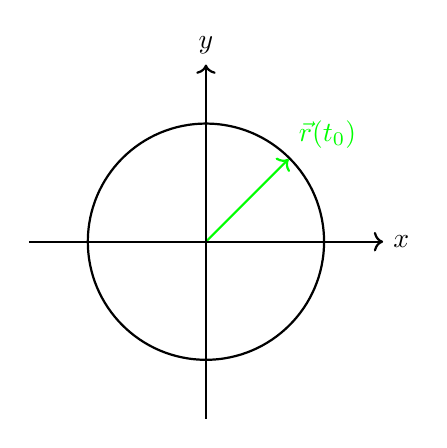
\begin{tikzpicture}[scale=1.5]
			% Draw the circle
			\draw[thick] (0, 0) circle (1);

			% Draw the radius vector
			\draw[->, thick, green] (0, 0) -- (0.7, 0.7) node[above right] {\(\vec{r}(t_0)\)};

			% Draw and label the axes
			\draw[->, thick] (-1.5, 0) -- (1.5, 0) node[right] {$x$};
			\draw[->, thick] (0, -1.5) -- (0, 1.5) node[above] {$y$};
		\end{tikzpicture}
	\end{minipage}%
	\hfill
	\begin{minipage}{0.45\textwidth}
		\centering
		\subsection*{3D Sphere}
		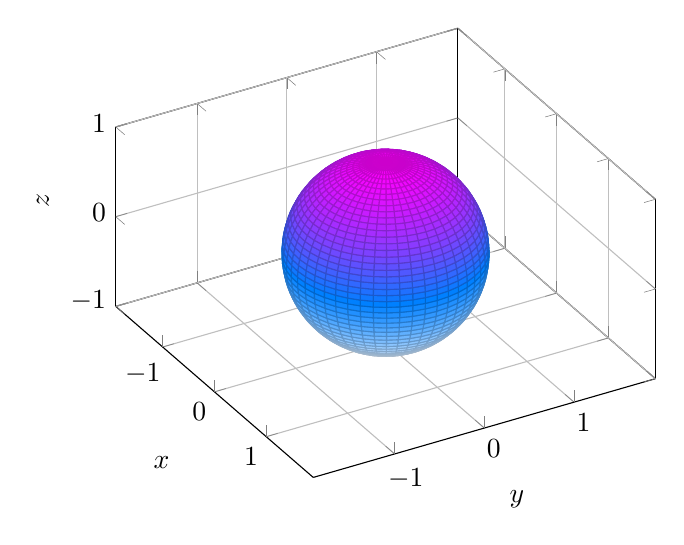
\begin{tikzpicture}
			\begin{axis}[
					xlabel={$x$},
					ylabel={$y$},
					zlabel={$z$},
					view={60}{30},
					grid=both,
					domain=-1:1,
					zmin=-1, zmax=1,
					axis equal,
				]
				% Use spherical coordinates to draw a sphere
				\addplot3[
					surf,
					colormap/cool,
					domain=0:360,
					domain y=0:180,
					samples=50,
					samples y=50,
					z buffer=sort
				]
				({sin(y)*cos(x)}, {sin(y)*sin(x)}, {cos(y)});
			\end{axis}
		\end{tikzpicture}
	\end{minipage}
\end{center}

\subsection{Deriving the Perpendicularity}
Let \(\vec{v}(t) = \vec{r}'(t)\) be the velocity vector. Then:
\[
	\vec{r}'(t) \cdot \vec{v}(t) = \vec{r}'(t) \cdot \vec{r}'(t) = \frac{1}{2} \frac{d}{dt} \left( \vec{r} \cdot \vec{r} \right).
\]
Differentiating:
\[
	= \frac{1}{2} \frac{d}{dt} \left( |\vec{r}'(t)|^2 \right) = \frac{1}{2} \frac{d}{dt} C^2 = 0,
\]
since \(C\) is constant.

Therefore, if \(\left| \vec{r}'(t) \right| = C\), then:
\[
	\vec{v}(t) \perp \vec{r}(t).
\]

\section{Calculating Curvature}

\subsection{Case 1: $\vec{r}(t)$ travels at unit speed around a circle}

We consider the position vector $\vec{r}(t)$ traveling at unit speed around a circle of radius $R$.

\[
	\vec{r}(t) = \left\langle R \cos\left(\frac{t}{R}\right), R \sin\left(\frac{t}{R}\right), 0 \right\rangle
\]

The velocity vector $\vec{v}(t)$ is then the derivative of the position vector:

\[
	\vec{v}(t) = \vec{r}'(t) = \left\langle -\sin\left(\frac{t}{R}\right), \cos\left(\frac{t}{R}\right), 0 \right\rangle
\]

Note that the magnitude of the velocity vector is 1 (unit speed):

\[
	|\vec{v}(t)| = 1
\]

The acceleration vector $\vec{a}(t)$, which is the second derivative of the position vector, is given by:

\[
	\vec{a}(t) = \vec{r}''(t) = \left\langle -\frac{1}{R} \cos\left(\frac{t}{R}\right), -\frac{1}{R} \sin\left(\frac{t}{R}\right), 0 \right\rangle
\]

\dfn{The curvature $\kappa(t)$ of the circle }{

	The magnitude of the acceleration vector (centripetal acceleration) is:

	\[
		\kappa(t) = |\vec{r}''(t)| = \frac{1}{R}
	\]

}

\begin{center}
	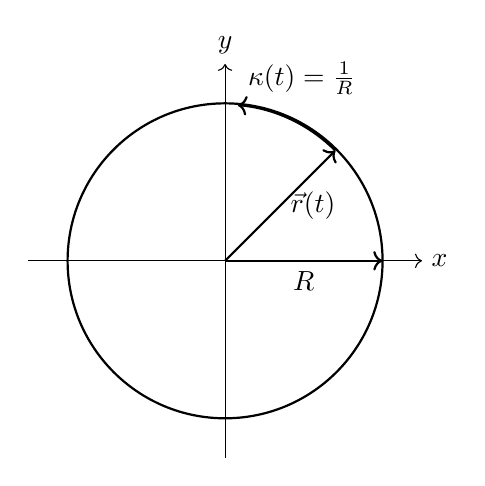
\begin{tikzpicture}
		% Circle
		\draw[thick] (0,0) circle (2);
		\draw[thick, ->] (0,0) -- (2,0) node[midway, below] {$R$};
		\draw[thick, ->] (0,0) -- (1.4,1.4) node[midway, right] {$\vec{r}(t)$};
		% Axes
		\draw[->] (-2.5,0) -- (2.5,0) node[right] {$x$};
		\draw[->] (0,-2.5) -- (0,2.5) node[above] {$y$};
		\draw[->, thick] (1.4,1.4) arc (45:85:2.0) node[above right] {$\kappa(t) = \frac{1}{R}$};
	\end{tikzpicture}
\end{center}

\nt{
	\begin{itemize}
		\item $\vec{r}(t)$ represents the position of a point moving around a circle of radius $R$.
		\item The velocity vector $\vec{v}(t)$ is orthogonal to $\vec{r}(t)$ and has a constant magnitude, indicating uniform circular motion.
		\item The acceleration vector $\vec{a}(t)$ points towards the center of the circle (centripetal acceleration) and its magnitude is inversely proportional to the radius $R$, showing that a smaller radius corresponds to a greater acceleration.
		\item The curvature $\kappa(t)$ is defined as the reciprocal of the radius of the circle, $\frac{1}{R}$.
	\end{itemize}
}

\subsection{Case 2: General Curve with Unit Speed}

Consider a curve given by the position vector $\vec{r}(t)$, which travels at unit speed along a general curve. This means that the magnitude of the velocity vector is constant:
\[
	|\vec{v}(t)| = 1.
\]
Since the speed is constant, the acceleration vector $\vec{a}(t)$ is orthogonal to the velocity vector:
\[
	\vec{v}(t) \cdot \vec{a}(t) = 0.
\]

This implies that all changes in $\vec{a}(t)$ are perpendicular to the direction of motion (velocity), which aligns with the properties of motion at unit speed.

\clm{Acceleration and the Osculating Circle}{}{
	The acceleration vector $\vec{a}(t)$ is directed towards the center of curvature of the curve at each point, and its magnitude is related to the curvature. In fact, the acceleration "matches" the behavior of the osculating circle at that point. The osculating circle is the circle that best approximates the curve locally, and its radius of curvature $R$ is inversely proportional to the curvature.
}

\thm{Curvature and Acceleration}{

	The curvature $\kappa(t)$ of the curve at time $t$ is defined as the magnitude of the acceleration vector:
	\[
		\kappa(t) = |\vec{a}(t)|.
	\]

	This provides a measure of how sharply the curve is bending at any given point. Since the speed is unitary, the curvature directly corresponds to the acceleration's magnitude.

}

\ex{Matching the Curve with Its Osculating Circle}{

	The osculating circle at a point on the curve is chosen so that its first and second derivatives match the curve's first and second derivatives, respectively:
	\[
		\text{Choose circle } \vec{C}(t) \text{ such that } \vec{C}'(t) \text{ and } \vec{C}''(t) \text{ match } \vec{r}'(t) \text{ and } \vec{r}''(t).
	\]

	This ensures that the circle is the best local approximation to the curve at that point, providing insight into the curve's behavior through the curvature.

}


\subsection{Case 3: General Curve with Variable Speed}

In this case, we analyze a general curve with a variable speed. Unlike the previous case, the magnitude of the velocity vector is not constant:
\[
	|\vec{v}(t)| \neq 1.
\]

This implies that the curve's speed is not uniform, and therefore, the analysis of the curvature will require a different approach.

\par

Let \( s(t) \) be the arc length parameter, which is a function of \( t \). The position vector can be reparameterized in terms of arc length:
\[
	\vec{r}(s^{-1}(t)),
\]
where \( s^{-1}(t) \) is the inverse function of \( s(t) \).

\thm{Calculating Curvature \( \kappa(t) \)}{

To find the curvature, we introduce a parameter \( t_0 \), which satisfies \( t_0 = s^{-1}(t) \). Thus, we have:
\[
	s^{-1}(t_0) = t.
\]
The curvature \( \kappa(t) \) is then given by:
\[
	\kappa(t) = \left| \frac{d}{d t_0} \vec{T}(s^{-1}(t_0)) \right|,
\]
where \( \vec{T}(t) \) is the unit tangent vector.

This can be rewritten as:
\[
\kappa(t) = \left| \frac{\frac{d}{d t} \vec{r}(s^{-1}(t))}{|\vec{r}'(s^{-1}(t))|} \right| = \left| \frac{\vec{T}'(s^{-1}(t_0))}{|\vec{r}'(s^{-1}(t_0))|} \right|.
	\]

	The final expression for the curvature is:
	\[
		\boxed{\kappa(t) = \frac{|\vec{T}'(t)|}{|\vec{r}'(t)|}}
	\]
	where \( \vec{T}(t) = \frac{\vec{r}'(t)}{|\vec{r}'(t)|} \) is the unit tangent vector to the curve. \\
	Alternatively, the curvature can be found with

	\[
		\boxed{\kappa (t) = \frac{\lvert \vec{a} \times \vec{v} \rvert}{\lvert \vec{v} \rvert^3}, \quad \kappa (t) = \frac{1}{\lvert \vec{v} \rvert} \left\lvert \frac{d\vec{T}}{dt} \right\rvert, \quad \kappa (t) = \lvert \frac{d\vec{T}}{ds} \rvert}
	\]

	if \(y = f(x)\)  can be parametrized as
	\[
		\vec{r}(t) = \langle t, f(t), 0 \rangle,
	\]
	where
	\[
		x'(t) = 1, \quad x''(t) = 0.
	\]
	This parametrization gives the curvature \(\kappa\) of the curve as
	\[
		\boxed{\kappa (t)= \frac{\lvert y''(x) \rvert}{\left( 1 + (y'(x))^2 \right)^{3/2}}.}
	\]
}

\section{Components of Acceleration}


\begin{center}
	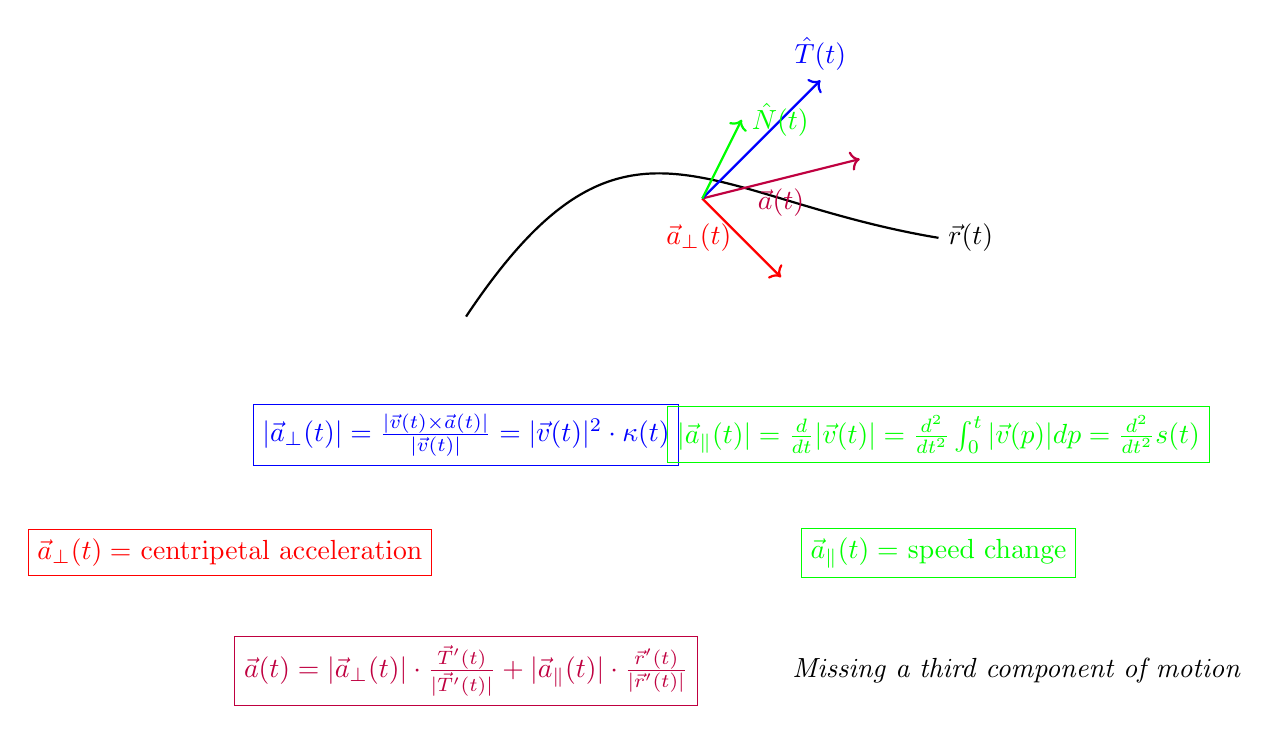
\begin{tikzpicture}

		% Curve and points
		\draw[thick] (0,0) .. controls (2,3) and (3,1.5) .. (6,1);
		\node[right] at (6,1) {$\vec{r}(t)$};

		% Acceleration vector and components
		\draw[->, thick, purple] (3,1.5) -- (5,2) node[midway, below] {$\vec{a}(t)$};
		\draw[->, thick, red] (3,1.5) -- (4,0.5) node[midway, left] {$\vec{a}_\perp(t)$};

		% Tangent and normal vectors
		\draw[->, thick, blue] (3,1.5) -- (4.5,3) node[above] {$\hat{T}(t)$};
		\draw[->, thick, green] (3,1.5) -- (3.5,2.5) node[right] {$\hat{N}(t)$};

		% Descriptive text boxes
		\node[draw=blue, text=blue] at (0,-1.5) {$|\vec{a}_\perp(t)| = \frac{|\vec{v}(t) \times \vec{a}(t)|}{|\vec{v}(t)|} = |\vec{v}(t)|^2 \cdot \kappa(t)$};
		\node[draw=green, text=green] at (6,-1.5) {$|\vec{a}_\parallel(t)| = \frac{d}{dt}|\vec{v}(t)| = \frac{d^2}{dt^2} \int_0^t |\vec{v}(p)| dp = \frac{d^2}{dt^2} s(t)$};

		% Labels for centripetal and speed change
		\node[draw=red, text=red] at (-3,-3) {$\vec{a}_\perp(t) =$ centripetal acceleration};
		\node[draw=green, text=green] at (6,-3) {$\vec{a}_\parallel(t) =$ speed change};

		% Final equation box
		\node[draw=purple, text=purple] at (0,-4.5) {$\vec{a}(t) = |\vec{a}_\perp(t)| \cdot \frac{\vec{T}'(t)}{|\vec{T	}'(t)|} + |\vec{a}_\parallel(t)| \cdot \frac{\vec{r}'(t)}{|\vec{r}'(t)|}$};

		% Comment on missing component
		\node[align=left] at (7,-4.5) {\textit{Missing a third component of motion}};
	\end{tikzpicture}
\end{center}


\section{Binormal Vector}
\dfn{Binormal Vector}{
	The \textbf{binormal vector} $\vec{B}$ is defined as:
	\[
		\vec{B} = \vec{T} \times \vec{N} = \frac{\vec{v} \times \vec{a}}{|\vec{v} \times \vec{a}|}
	\]
	where:
	\begin{itemize}
		\item $\vec{T}$ is the unit tangent vector to the curve, given by:
		      \[
			      \vec{T} = \frac{\vec{r}'(t)}{|\vec{r}'(t)|}
		      \]
		\item $\vec{N}$ is the unit normal vector to the curve, and it is defined as:
		      \[
			      \vec{N} = \frac{\vec{T}'(t)}{|\vec{T}'(t)|}
		      \]
	\end{itemize}
	The binormal vector $\vec{B}$ represents the direction to exit the current plane of motion described by the vectors $\vec{T}$ and $\vec{N}$.
}

\subsection{Change in the Plane of Motion}

The rate of change of the binormal vector is given by:
\[
	\frac{d\vec{B}}{dt} = \text{change in the plane of motion}
\]

Applying the derivative product rule to $\vec{B} = \vec{T} \times \vec{N}$:
\[
	\frac{d}{dt} (\vec{T} \times \vec{N}) = \frac{d\vec{T}}{dt} \times \vec{N} + \vec{T} \times \frac{d\vec{N}}{dt}
\]
Since:
\[
	\vec{N} = \frac{\vec{T}'(t)}{|\vec{T}'(t)|}
\]
it follows that:
\[
	\vec{T} \cdot \vec{N} = 0
\]
and thus:
\[
	\frac{d\vec{B}}{dt} \text{ is orthogonal to both } \vec{T} \text{ and } \vec{N}
\]

\subsection{Torsion and its Relation to the Binormal Vector}

Since $\vec{N}$ is a unit vector, the vector $\vec{B}'$ is parallel to $\vec{N}$:
\[
	\frac{d\vec{B}}{dt} = -\tau \vec{N}
\]
where $\tau$ is the \textbf{torsion} of the plane of movement.

\nt{
	If $\tau > 0$, the motion is on the plane of movement; if $\tau < 0$, the motion is in the opposite direction.
}

To find $\tau$, take the dot product of both sides with $\vec{N}$:
\[
	\frac{d\vec{B}}{dt} \cdot \vec{N} = -\tau (\vec{N} \cdot \vec{N}) = -\tau
\]
Thus, at unit speed:
\dfn{Torsion $\tau$ at unit speed}{
	\[
		\tau = -\frac{\frac{d\vec{B}}{dt} \cdot \vec{N}}{|\vec{N}|} = -\frac{d\vec{B}}{dt} \cdot \vec{N}
	\]
}

\subsection{General Case and Torsion Formula}

For the general case, replace $\vec{r}(t)$ with $\vec{r}(s^{-1}(t))$, where $s(t)$ is the arc-length parameterization.

The derivative of $\vec{B}$ in the general case is given by:
\[
	\frac{d\vec{B}(s^{-1})}{d(t_0)} = \frac{\vec{B}'(s^{-1}(t_0))}{|\vec{r}'(s^{-1}(t_0))|}
\]
or simply:
\[
	\frac{d\vec{B}(t)}{dt} = \frac{\vec{B}'(t) \cdot \vec{N}(t)}{|\vec{r}'(t)|}
\]
The general formula for torsion $\tau$ becomes:

\dfn{General form for torsion $\tau$}{
	\[
		\tau = \frac{\vec{B}'(t) \cdot \vec{N}(t)}{|\vec{r}'(t)|}
	\]
	.
}

\subsection{Expressing the Binormal Vector with Velocity and Acceleration}

The binormal vector $\vec{B}$ can be expressed as:
\[
	\vec{B} = \frac{\vec{v} \times \vec{a}}{|\vec{v} \times \vec{a}|}
\]
where $\vec{v}$ is the velocity vector and $\vec{a}$ is the acceleration vector.

The torsion $\tau$ is given by:
\[
	\tau = \frac{(\vec{v} \times \vec{a}) \cdot \vec{a}'}{|\vec{v} \times \vec{a}|^2}
\]

\nt{
	The centripetal acceleration determines the curvature of the path.
}
\ex{Finding the Torsion of a Helix Path}{

	Consider the helix parameterized by:
	\[
		\vec{r}(t) = \langle \cos t, \sin t, t \rangle
	\]

	The first derivative (velocity vector) is:
	\[
		\vec{r}'(t) = \langle -\sin t, \cos t, 1 \rangle
	\]
	with magnitude:
	\[
		|\vec{r}'(t)| = \sqrt{2}
	\]

	The unit tangent vector $\vec{T}(t)$ is:
	\[
		\vec{T}(t) = \frac{\vec{r}'(t)}{|\vec{r}'(t)|} = \left\langle -\frac{\sin t}{\sqrt{2}}, \frac{\cos t}{\sqrt{2}}, \frac{1}{\sqrt{2}} \right\rangle
	\]

	The derivative of the tangent vector is:
	\[
		\vec{T}'(t) = \left\langle -\frac{\cos t}{\sqrt{2}}, -\frac{\sin t}{\sqrt{2}}, 0 \right\rangle
	\]
	and its magnitude is:
	\[
		|\vec{T}'(t)| = \frac{1}{\sqrt{2}}
	\]

	The curvature $\kappa(t)$ is given by:
	\[
		\kappa(t) = \frac{|\vec{T}'(t)|}{|\vec{r}'(t)|} = \frac{\frac{1}{\sqrt{2}}}{\sqrt{2}} = \frac{1}{2}
	\]
	Hence, the radius of curvature $R(t)$ is:
	\[
		R(t) = \frac{1}{\kappa(t)} = 2
	\]

	The normal vector $\vec{N}(t)$ is:
	\[
		\vec{N}(t) = \frac{\vec{T}'(t)}{|\vec{T}'(t)|} = \left\langle -\cos t, -\sin t, 0 \right\rangle
	\]
	which points towards the center of the curvature.

	The normal acceleration $a_N$ is:
	\[
		a_N = |\vec{r}'(t)|^2 \cdot \kappa = 1 \quad \text{(constant, points towards the center)}
	\]

	The tangential acceleration is:
	\[
		a_T = s''(t), \quad s(t) = t \sqrt{2}, \quad s'(t) = \sqrt{2}
	\]

	The binormal vector $\vec{B}$ is given by:
	\[
		\vec{B} = \vec{T} \times \vec{N} = \frac{1}{\sqrt{2}} \langle \sin t, -\cos t, 0 \rangle
	\]

	The derivative of the binormal vector is:
	\[
		\vec{B}' = \frac{1}{\sqrt{2}} \langle \cos t, \sin t, 0 \rangle = -\frac{1}{\sqrt{2}} \vec{N} \implies \tau = \frac{\vec{B}' \cdot \vec{N}}{|\vec{r}'(t)|} = \frac{1}{2}
	\]

	Therefore, the torsion $\tau$ is:
	\[
		\tau = \frac{\kappa}{\sqrt{2}} = \frac{1}{2}
	\]

}

\chapter{Functions of Multiple Random Variables $f:\mathbb{R} ^ n \rightarrow \mathbb{R}$}

\section{Plotting Multiple Random Variable Functions}

Consider a function $f(x, y) = z$. We aim to plot functions in 3D.

\subsection*{Example}
\[
	f(x, y) = x^2 + y^2
\]

\begin{itemize}
	\item When $y = 0$, $f(x, 0) = x^2$.
	\item When $x = 0$, $f(0, y) = y^2$.
\end{itemize}

\begin{center}
	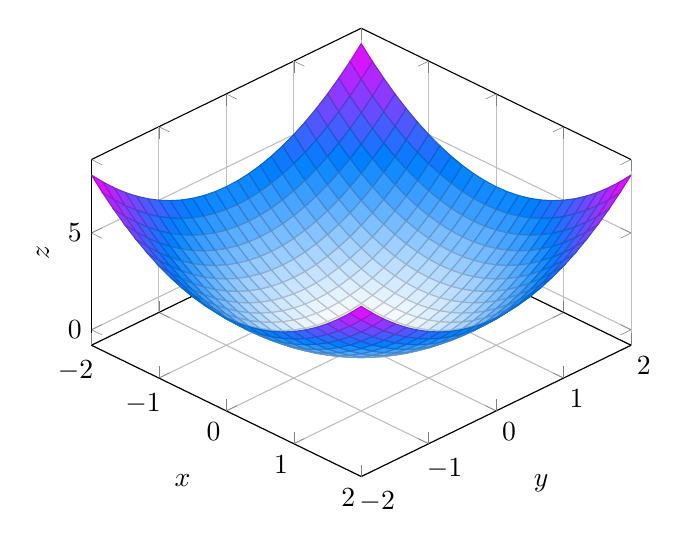
\begin{tikzpicture}
		\begin{axis}[
				view={45}{45},
				xlabel={$x$},
				ylabel={$y$},
				zlabel={$z$},
				grid=major,
				colormap/cool,
			]
			\addplot3[surf, domain=-2:2, domain y=-2:2]
			{x^2 + y^2};
		\end{axis}
	\end{tikzpicture}
\end{center}

For this surface:
\begin{itemize}
	\item If $z = 0$, $(x, y) = (0, 0)$.
	\item If $z = 1$, $x^2 + y^2 = 1$, which represents a \textbf{circle}.
	\item If $z > 0$, $x^2 + y^2 = z$, representing a circle with radius $\sqrt{z}$ in the $xy$-plane.
\end{itemize}

The vertical line test still applies: a vertical line intersects the surface at at most 1 point.

\begin{center}
	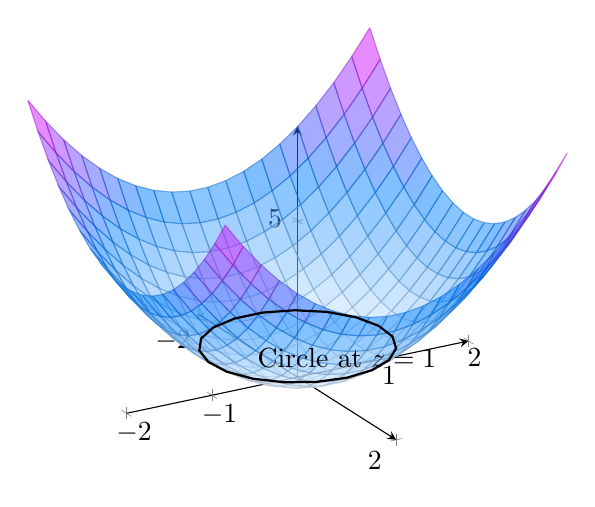
\begin{tikzpicture}
		\begin{axis}[
				axis lines = middle,
				domain=-2:2,
				y domain=-2:2,
				view={60}{30},
				samples=20,
				samples y=20,
				colormap/cool,
			]
			\addplot3[surf, opacity=0.5] {x^2 + y^2};
			\addplot3[thick, domain=0:2*pi, samples y=0]
			({cos(deg(x))}, {sin(deg(x))}, {1}) node[above] {Circle at $z = 1$};
		\end{axis}
	\end{tikzpicture}
\end{center}

\subsection*{Sphere by Self Equation}

A sphere cannot be represented as a function in the form $f(x, y) = z$. This is because it fails the vertical line test; a vertical line may intersect the sphere at multiple points.

\begin{center}
	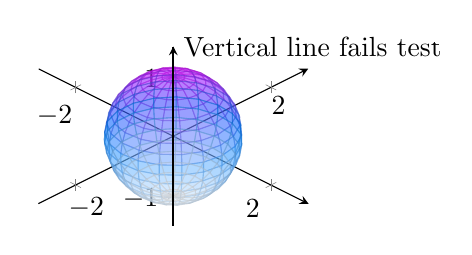
\begin{tikzpicture}
		\begin{axis}[
				axis lines = middle,
				view={45}{30},
				grid=major,
				axis equal
			]
			% Draw the sphere using parametric equations
			\addplot3[
				surf,
				domain=0:360,
				y domain=0:180,
				samples=20,
				samples y=20,
				opacity=0.4,
				colormap/cool,
			]
			({sin(y)*cos(x)}, {sin(y)*sin(x)}, {cos(y)});
			% Vertical line test
			\addplot3[
				thick,
				domain=-1.5:1.5,
				samples y=0,
			]
			({0}, {0}, {x}) node[right] {Vertical line fails test};
		\end{axis}
	\end{tikzpicture}
\end{center}

\section{Domain of Multiple Random Variable Functions}


\dfn{Domain}{The domain of $f(x, y)$ is the set of pairs $(x, y) \in \mathbb{R}^2$ such that $f(x, y)$ is defined.}
\ex{Example of finding domain}{
	Let
	\[
		f(x, y) = \sqrt{4 - x^2 - y^2}
	\]
	To ensure that $f(x, y)$ is defined, the expression inside the square root must be non-negative:
	\[
		4 - x^2 - y^2 \geq 0 \implies x^2 + y^2 \leq 4
	\]

	This inequality describes a disk of radius 2 centered at the origin $(0, 0)$.

	\begin{center}
		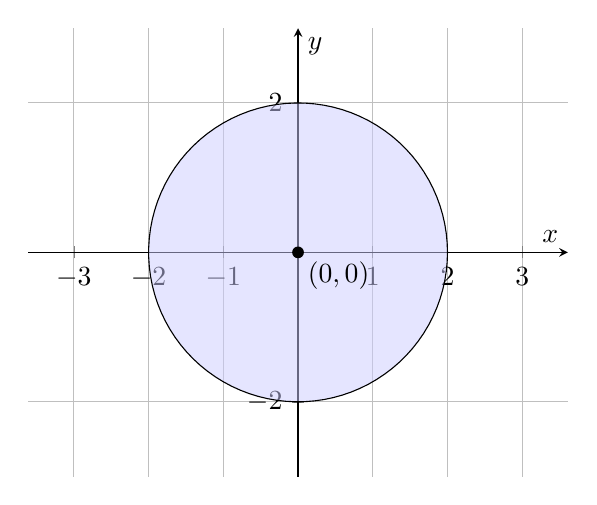
\begin{tikzpicture}
			% Draw the domain as a disk
			\begin{axis}[
					axis equal,
					xlabel = {$x$},
					ylabel = {$y$},
					axis lines = middle,
					xmin = -3, xmax = 3,
					ymin = -3, ymax = 3,
					grid = major
				]
				% Disk with radius 2
				\addplot[draw=black, fill=blue!20, fill opacity=0.5, domain=0:2*pi, samples=100]
				({2*cos(deg(x))}, {2*sin(deg(x))});
				% Origin marker
				\node at (axis cs:0, 0) [circle, fill=black, inner sep=1.5pt] {};
				\node[below right] at (axis cs:0, 0) {$(0, 0)$};
			\end{axis}
		\end{tikzpicture}
	\end{center}

	Therefore, the domain of $f(x, y)$ is:
	\[
		\{(x, y) \in \mathbb{R}^2 \mid x^2 + y^2 \leq 4\}
	\]
}


\section{Range of Multiple Random Variable Functions}

\dfn{Range}{
	The range of a function $f(x, y)$ is the set of all $z$ such that $z = f(x, y)$ for some input $(x, y)$.
}

\ex{Example of finding the range}{
	Consider the function
	\[
		f(x, y) = \sqrt{4 - x^2 - y^2}
	\]
	Evaluating $f$ at the origin:
	\[
		f(0, 0) = \sqrt{4 - 0^2 - 0^2} = 2
	\]
	The maximum value of $f$ is 2. To find the minimum, consider the boundary of the domain:
	If $x^2 + y^2 = 4$, then
	\[
		f(x, y) = \sqrt{4 - (x^2 + y^2)} = \sqrt{4 - 4} = 0
	\]

	Therefore, the range of $f(x, y)$ is:
	\[
		\{ z \in [0, 2] \}
	\]
}

\ex{Another example}{
	Let
	\[
		f(x, y) = x^2 + y^2
	\]
	Since $f(x, y) \geq 0$ for all $(x, y) \in \mathbb{R}^2$, the range of $f(x, y)$ is:
	\[
		\{ z \mid z \geq 0 \}
	\]
}

\section{Level Curves of Functions of Two Variables}

\dfn{Level Curves}{
	Level curves (or contour lines) of a function $f(x, y)$ are curves in the $xy$-plane along which the function takes a constant value. For a given value $c$, a level curve is the set of points $(x, y)$ such that:
	\[
		f(x, y) = c
	\]
}

\ex{Example of level curves}{
	Consider the function:
	\[
		f(x, y) = x^2 + y^2
	\]
	To find the level curves for this function, set $f(x, y)$ equal to a constant $c$:
	\[
		x^2 + y^2 = c
	\]
	These curves are circles centered at the origin with radius $\sqrt{c}$.

	\begin{center}
		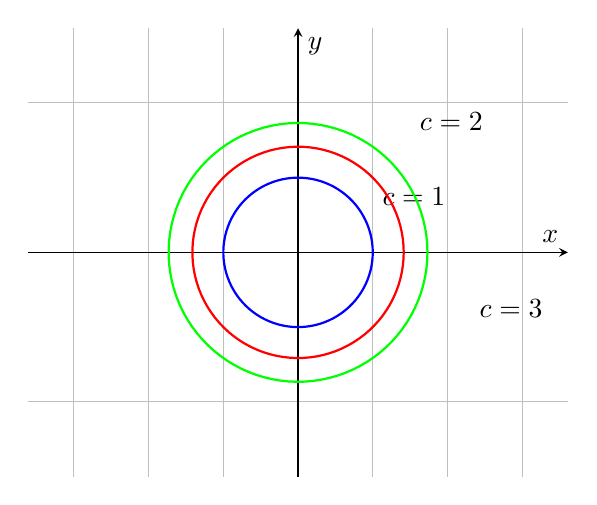
\begin{tikzpicture}
			% Draw level curves as circles
			\begin{axis}[
					axis equal,
					xlabel = {$x$},
					ylabel = {$y$},
					axis lines = middle,
					xmin = -3, xmax = 3,
					ymin = -3, ymax = 3,
					grid = major,
					ticks=none
				]
				% Level curve for c = 1
				\addplot[blue, thick, domain=0:2*pi, samples=100]
				({sqrt(1)*cos(deg(x))}, {sqrt(1)*sin(deg(x))});
				\node[above right] at (axis cs: 1, 0.5) {$c = 1$};

				% Level curve for c = 2
				\addplot[red, thick, domain=0:2*pi, samples=100]
				({sqrt(2)*cos(deg(x))}, {sqrt(2)*sin(deg(x))});
				\node[above right] at (axis cs: 1.5, 1.5) {$c = 2$};

				% Level curve for c = 3
				\addplot[green, thick, domain=0:2*pi, samples=100]
				({sqrt(3)*cos(deg(x))}, {sqrt(3)*sin(deg(x))});
				\node[below right] at (axis cs: 2.3, -0.5) {$c = 3$};
			\end{axis}
		\end{tikzpicture}
	\end{center}


	In this case, each level curve is a circle centered at the origin. The radius of each circle is $\sqrt{c}$, indicating that as the value of $c$ increases, the radius of the level curve also increases.

}

\section{Limits of Two-Variable Functions}

\dfn{Limit of a Two-Variable Function}{
	Let $f(x, y)$ be a function of two variables. The limit of $f(x, y)$ as $(x, y)$ approaches $(a, b)$ is denoted as:
	\[
		\lim_{(x, y) \to (a, b)} f(x, y) = L
	\]
	This means that as the point $(x, y)$ gets arbitrarily close to $(a, b)$, the function values $f(x, y)$ approach the value $L$. For the limit to exist, the function must approach the same value $L$ regardless of the path taken to reach $(a, b)$.
}

\dfn{Formal Definition}{

	\[
		\lim_{(x,y) \to (a,b)} f(x,y) = L
	\]
	if for any \( \varepsilon > 0 \), there exists a constant \( \delta > 0 \) such that:
	\[
		|f(x,y) - L| < \varepsilon
	\]
	whenever \( (x, y) \) are in the domain of \( f \) and:
	\[
		|(x,y) - (a,b)| < \delta
	\]

}

\subsection*{Visualizing Limits}

The concept of limits for two-variable functions can be visualized in 3D, where $f(x, y)$ is represented as a surface over the $xy$-plane. The behavior of the function as $(x, y)$ approaches a point $(a, b)$ corresponds to how the surface approaches a specific height, $L$.

\begin{center}
	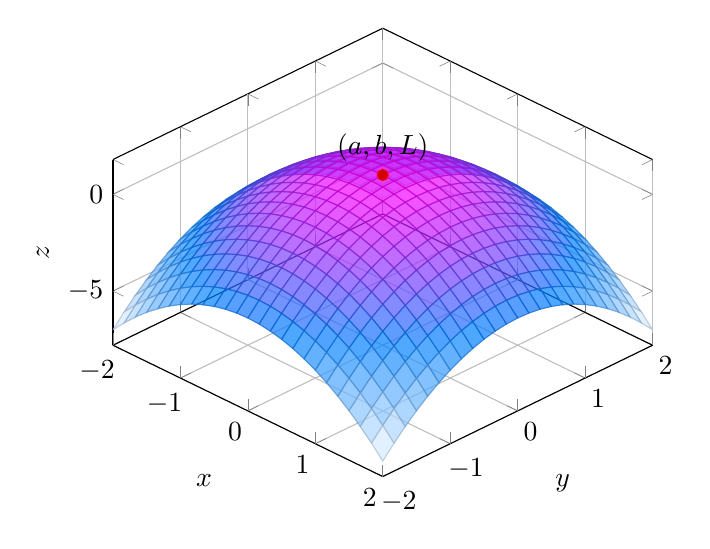
\begin{tikzpicture}
		\begin{axis}[
				view={45}{45},
				xlabel={$x$},
				ylabel={$y$},
				zlabel={$z$},
				domain=-2:2,
				domain y=-2:2,
				grid=major,
				colormap/cool,
			]
			% A sample function to visualize limit
			\addplot3[surf, opacity=0.7] {1 - (x^2 + y^2)};
			\addplot3+[mark=*, only marks] coordinates {(0,0,1)};
			\node at (axis cs: 0, 0, 1.2) [above] {$(a, b, L)$};
		\end{axis}
	\end{tikzpicture}
\end{center}

In this diagram, the surface represents a function $f(x, y)$, and the point $(a, b, L)$ is the limit we are trying to approach.

\ex{Example of a Limit}{
	Consider the function:
	\[
		f(x, y) = \frac{x^2 - y^2}{x^2 + y^2}
	\]
	We want to find
	\[
		\lim_{(x, y) \to (0, 0)} f(x, y)
	\]

	Evaluating the limit along different paths:
	\begin{itemize}
		\item Along the path $y = 0$, we have $f(x, 0) = \frac{x^2}{x^2} = 1$.
		\item Along the path $x = 0$, we have $f(0, y) = \frac{-y^2}{y^2} = -1$.
	\end{itemize}

	Since the limit depends on the path taken to approach $(0, 0)$, the limit does not exist.

	\begin{center}
		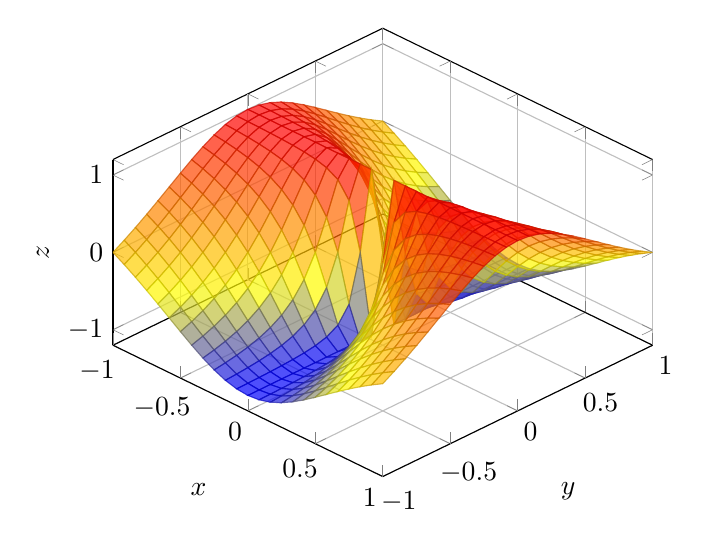
\begin{tikzpicture}
			\begin{axis}[
					view={45}{45},
					xlabel={$x$},
					ylabel={$y$},
					zlabel={$z$},
					domain=-1:1,
					domain y=-1:1,
					grid=major,
					colormap/hot,
				]
				% The surface of the function to visualize path-dependent behavior
				\addplot3[surf, opacity=0.7] {(x^2 - y^2)/(x^2 + y^2)};
			\end{axis}
		\end{tikzpicture}
	\end{center}

	This diagram shows how the function behaves differently along different paths toward the origin, resulting in no single limit.

}

\ex{Example of a Limit that Exists}{
	Consider the function:
	\[
		f(x, y) = x^2 + y^2
	\]
	We want to find
	\[
		\lim_{(x, y) \to (0, 0)} f(x, y)
	\]

	Since $f(x, y) = x^2 + y^2$, regardless of the path taken to approach $(0, 0)$, the value of $f(x, y)$ approaches $0$. Therefore,
	\[
		\lim_{(x, y) \to (0, 0)} f(x, y) = 0.
	\]

	\begin{center}
		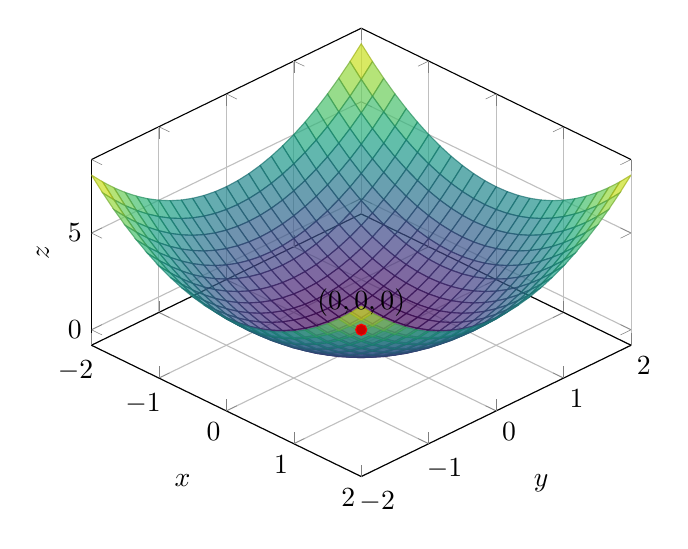
\begin{tikzpicture}
			\begin{axis}[
					view={45}{45},
					xlabel={$x$},
					ylabel={$y$},
					zlabel={$z$},
					domain=-2:2,
					domain y=-2:2,
					grid=major,
					colormap/viridis,
				]
				% A simple surface where the limit exists
				\addplot3[surf, opacity=0.7] {x^2 + y^2};
				\addplot3+[mark=*, only marks] coordinates {(0,0,0)};
				\node at (axis cs: 0, 0, 0.2) [above] {$(0, 0, 0)$};
			\end{axis}
		\end{tikzpicture}
	\end{center}

}

\subsection{Limits by substituting with function $f:\mathbb{R} \rightarrow \mathbb{R}$}

\ex{Changing $g(x)$}{

	For a function $f(x, y)$, the limit as $(x, y)$ approaches a point $(a, b)$ must be the same regardless of the path taken to approach $(a, b)$.

	Consider the function:
	\[
		f(x, y) = \frac{3xy^2}{x^2 + y^4}
	\]
	We wish to find:
	\[
		\lim_{(x, y) \to (0, 0)} f(x, y)
	\]
	This limit initially appears to be of the form $\frac{0}{0}$, indicating an indeterminate form.

	To proceed, we evaluate the limit along different paths. Let’s test two paths to see if the limit is consistent.

	\subsection*{Path 1: Linear Path $y = mx$}
	Substitute $y = mx$ into $f(x, y)$:
	\[
		f(x, y) = \frac{3x(mx)^2}{x^2 + (mx)^4} = \frac{3m^2 x^3}{x^2 + m^4 x^4}
	\]
	Then, consider the limit as $x \to 0$:
	\[
		\lim_{x \to 0} \frac{3m^2 x^3}{x^2 + m^4 x^4}
	\]
	Factor out $x^2$ in the denominator:
	\[
		= \lim_{x \to 0} \frac{3m^2 x}{1 + m^4 x^2} = 0
	\]

	\subsection*{Path 2: Parabolic Path $y = m\sqrt{x}$}
	Substitute $y = m\sqrt{x}$ into $f(x, y)$:
	\[
		f(x, y) = \frac{3x(m\sqrt{x})^2}{x^2 + (m\sqrt{x})^4} = \frac{3m^2 x^2}{x^2 + m^4 x^2}
	\]
	Then, consider the limit as $x \to 0$:
	\[
		\lim_{x \to 0} \frac{3m^2 x^2}{(m^4 + 1)x^2} = \lim_{x \to 0} \frac{3m^2}{m^4 + 1} = \frac{3m^2}{m^4 + 1} \neq 0
	\]

	Since the limit depends on the path taken (0 for the linear path and $\frac{3m^2}{m^4 + 1}$ for the parabolic path), the limit does not exist:
	\[
		\lim_{(x, y) \to (0, 0)} f(x, y) \text{ DNE (Does Not Exist)}
	\]
}

\subsection{Limits by substituting with Vector Valued Functions $f:\mathbb{R} \rightarrow \mathbb{R}^n$}

\ex{Substituting $< g_1(t), g_2(t) > $}{
	Since a 1 to 1 function $g(t)$ must pass the vertical line test, it is a limiting way to approach the point at which we want to compute the limit of a two variable function. Using a vector valued function will remove this limitation and enable us to approach from any direction.

	For a function $f(x, y)$, the limit as $(x, y)$ approaches a point $(a, b)$ must be the same regardless of the path taken to approach $(a, b)$.

	Consider the function:
	\[
		f(x, y) = \frac{3xy^2}{x^2 + y^4}
	\]
	We wish to find:
	\[
		\lim_{(x, y) \to (0, 0)} f(x, y)
	\]
	This limit initially appears to be of the form $\frac{0}{0}$, indicating an indeterminate form.

	To proceed, we evaluate the limit along different paths. Let’s test two paths to see if the limit is consistent.

	\subsection*{Path 1: Parametric Linear Path $\vec{r}(t) = \langle t, mt \rangle$}

	Substitute $\vec{r}(t) = \langle t, mt \rangle$ into $f(x, y)$:
	\[
		f(x, y) = \frac{3(t)(mt)^2}{t^2 + (mt)^4} = \frac{3m^2 t^3}{t^2 + m^4 t^4}
	\]
	Then, consider the limit as $t \to 0$:
	\[
		\lim_{t \to 0} \frac{3m^2 t^3}{t^2 + m^4 t^4}
	\]
	Factor out $t^2$ in the denominator:
	\[
		= \lim_{t \to 0} \frac{3m^2 t}{1 + m^4 t^2} = 0
	\]

	\subsection*{Path 2: Parametric Parabolic Path $\vec{r}(t) = \langle t^2, m\sqrt{t} \rangle$}

	Substitute $\vec{r}(t) = \langle t^2, m\sqrt{t} \rangle$ into $f(x, y)$:
	\[
		f(x, y) = \frac{3(t^2)(m\sqrt{t})^2}{(t^2)^2 + (m\sqrt{t})^4} = \frac{3m^2 t^3}{t^4 + m^4 t^2}
	\]
	Then, consider the limit as $t \to 0$:
	\[
		\lim_{t \to 0} \frac{3m^2 t^3}{t^4 + m^4 t^2}
	\]
	Factor out $t^2$ in the denominator:
	\[
		= \lim_{t \to 0} \frac{3m^2 t}{t^2 + m^4} = \frac{3m^2}{m^4} = \frac{3}{m^2} \neq 0
	\]

	Since the limit depends on the path taken (0 for the linear path and $\frac{3}{m^2}$ for the parabolic path), the limit does not exist:
	\[
		\lim_{(x, y) \to (0, 0)} f(x, y) \text{ DNE (Does Not Exist)}
	\]

}

\ex{Other Example}{

	$$f(x,y)=\frac{\sqrt[2]{x+y} + ln(\sqrt[2]{x+y})}{x+y}$$

	\[
		f(x,y) =
		\begin{cases}
			\frac{\sqrt[2]{x+y} + ln(\sqrt[2]{x+y})}{x+y} & \text{if } x,y \neq 0 \\
			L                                             & \text{if } x=y=0      \\
		\end{cases}
	\]

	If

	$$g(t)=<g_1(t),g_2(t)>$$

	where $g_1(t) = t, g_2(t)=\sqrt{t}$

	and

	$$h(s) = \frac{\sqrt[2]{s} + ln(\sqrt[2]{s})}{s}$$

	then

	$$f(x,y) = h(g_1(x),g_2(y))$$

}

\section{Tips for Finding Limits of Two-Variable Functions (2VF)}

\subsection{Polynomials are Continuous}
Polynomials in two variables are always continuous everywhere in their domain. For example:
\[
	f(x, y) = 3x^2 + 2y^2 + 3x^4 + 1
\]
is continuous for all $(x, y) \in \mathbb{R}^2$.

\subsection{Compositions of Continuous Functions are Continuous}
If $g(t)$ is a function of one variable and continuous at $t = 0$, and $f(x, y)$ is a continuous function of two variables, then $g(f(x, y))$ is also continuous at any point where $f(x, y)$ is defined. For example:
\[
	g(t) =
	\begin{cases}
		\frac{\sqrt{1 + t} - 1}{t} & \text{if } t \neq 0 \\
		e                          & \text{if } t = 0
	\end{cases}
\]
is continuous everywhere.

Now consider the function:
\[
	f(x, y) = x y^2
\]
Since $f(x, y)$ is continuous, the composition $g(f(x, y))$ is also continuous. Specifically:
\[
	g(f(x, y)) =
	\begin{cases}
		\frac{\sqrt{1 + x y^2} - 1}{x y^2} & \text{if } x y^2 \neq 0 \\
		e                                  & \text{if } x y^2 = 0
	\end{cases}
\]
This composition is continuous.

\subsection{Rational Functions}
A rational function $f(x, y) = \frac{P(x, y)}{Q(x, y)}$ is continuous at all points where the denominator $Q(x, y) \neq 0$. For example:
\[
	f(x, y) = \frac{3x y^2}{x^2 + y^4}
\]
is continuous wherever $x^2 + y^4 \neq 0$.

\nt{\textbf{Tip on Factoring and Simplifying} \\
	To find the limit of a rational function, try factoring and simplifying the expression. This can help identify points of discontinuity or removable singularities.
}

\subsection{Special Limits: Squeeze Theorem}
The Squeeze Theorem can be used for two-variable functions. If:
\[
	h(x, y) \leq f(x, y) \leq g(x, y)
\]
and both $h(x, y)$ and $g(x, y)$ approach the same limit $L$ as $(x, y) \to (a, b)$, then:
\[
	\lim_{(x, y) \to (a, b)} f(x, y) = L
\]

\subsection{Use of Polar Coordinates}
For limits involving two-variable functions, converting to polar coordinates can often simplify the problem. Let:
\[
	x = r \cos \theta, \quad y = r \sin \theta
\]
Then, $f(x, y)$ becomes a function of $r$ and $\theta$, which can be easier to analyze as $r \to 0$. This is particularly useful when the limit depends on the distance from the origin.

\subsection{Testing Multiple Paths}
When checking if a limit exists, test multiple paths (e.g., $y = mx$, $y = m\sqrt{x}$, $x = 0$, $y = 0$). If the limit differs for any path, then the limit does not exist. However, if all paths give the same result, it is likely that the limit exists (though more thorough testing is required for rigor).

\subsection{Continuity of Common Functions}
Most standard functions (e.g., trigonometric, exponential, logarithmic) are continuous within their domains. If they are composed with continuous functions of $x$ and $y$, the result is continuous as well.

\subsection{Rational functions}
Consider a rational function of two variables in the form:

\[
	\frac{h(x, y)}{g(x, y)}
\]

where \( h(x, y) \) and \( g(x, y) \) are polynomials. The behavior of the limit of this function as \( (x, y) \to (a, b) \) can be classified into three cases:

\subsection{Case 1: \( g(a, b) \neq 0 \)}

If the denominator \( g(x, y) \) is non-zero at the point \( (a, b) \), i.e., \( g(a, b) \neq 0 \), then the function is continuous at \( (a, b) \). In this case, we have:

\[
	\lim_{(x, y) \to (a, b)} \frac{h(x, y)}{g(x, y)} = \frac{h(a, b)}{g(a, b)}.
\]

Thus, the limit exists and equals the value of the function at the point \( (a, b) \).

\subsection{Case 2: \( g(a, b) = 0 \) and \( h(a, b) \neq 0 \)}

If the denominator \( g(x, y) \) equals zero at \( (a, b) \) but the numerator \( h(x, y) \) does not, i.e., \( h(a, b) \neq 0 \), then the limit does not exist. Intuitively, this is because the denominator tends to zero while the numerator tends to a non-zero constant, leading to a blow-up of the function.

\[
	\lim_{(x, y) \to (a, b)} \frac{h(x, y)}{g(x, y)} \quad \text{does not exist}.
\]

\subsection{Case 3: \( h(a, b) = g(a, b) = 0 \)}

If both the numerator and the denominator are zero at \( (a, b) \), i.e., \( h(a, b) = g(a, b) = 0 \), we have an indeterminate form \( \frac{0}{0} \). In this case, we try to simplify the expression by factoring out the common terms in \( h(x, y) \) and \( g(x, y) \).

\ex{Example}{

	Consider the function:

	\[
		\frac{x^2 - y^2}{x - y}.
	\]

	At the point \( (1, 1) \), both the numerator and the denominator are zero:

	\[
		h(1, 1) = g(1, 1) = 0.
	\]

	We factor the numerator:

	\[
		x^2 - y^2 = (x - y)(x + y).
	\]

	Now, cancel the common factor \( x - y \) in the numerator and denominator:

	\[
		\frac{x^2 - y^2}{x - y} = x + y.
	\]

	Thus, the limit simplifies to:

	\[
		\lim_{(x, y) \to (1, 1)} \frac{x^2 - y^2}{x - y} = \lim_{(x, y) \to (1, 1)} (x + y) = 1 + 1 = 2.
	\]

	Hence, by removing the common factor, the limit can be computed as \( 2 \).
}

\subsection{Case 4: \( h(a, b) = g(a, b) = 0 \) still}

Try several Vector Valued functions, trying to make the denominator small or big compared to the numerator

\ex{Large denominator}{
	\[
		\quad \lim_{(x,y) \to (0,0)} \frac{x^2 y}{x^2 + y^2}
	\]
	One possible path: Let \( y = 0 \),
	\[
		\frac{x^2 (0)}{x^2 + 0^2} = \frac{0}{x^2} = 0
	\]

	Now try a different path: Let \( x = 0 \),
	\[
		\frac{0^2 y}{0^2 + y^2} = \frac{0}{y^2} = 0
	\]

	\noindent \textbf{Parametric form:}
	\[
		\lim_{t \to 0} f(r_1(t), r_2(t)) = \lim_{t \to 0} f(0,t) = \lim_{t \to 0} \frac{0^2 t}{0^2 + t^2} = \lim_{t \to 0} 0 = 0
	\]

	Thus, the limit is \( 0 = 0 \).
}

\ex{Small denominator}{

	\[
		x = -y^2 + y^n, \quad \text{where } n > 2
	\]
	(for \( y \) small)

	\[
		\lim_{t \to 0} f(t^2 + t^n, t) = \frac{(t^4 - 2t^{n+2} + t^{2n}) t}{t^2 + t^n + t^2} = \lim_{t \to 0} \frac{t^5 - 2t^{n+3} + t^{2n+1}}{t^n} \quad (n=5)
	\]
	Simplifying:
	\[
		n = 5: \quad \lim_{t \to 0} \left(1-2t^3 + t^6 \right) = 1
	\]

}

\subsection{Case 5: Still getting the same limit}

\ex{Trying}{
	Let $\lim_{(x,y) \to (0,0)} = \frac{xy^2}{x^2+y^2}$. \\
	If we divide by $y^2$ we get
	\[
		\lim_{(x, y) \to (0,0)} \frac{xy^2}{x^2+y^2} = \lim_{(x, y) \to (0,0)} \frac{x}{(\frac{x^2}{y^2})+1} = 0
	\]
}


\section{Properties of Limits of Two-Variable Functions}

Let $f(x, y)$ and $g(x, y)$ be two functions of two variables such that:
\[
	\lim_{(x, y) \to (a, b)} f(x, y) = L_1, \quad \lim_{(x, y) \to (a, b)} g(x, y) = L_2
\]
Then, the following properties hold:

\subsection{Scaling by a constant:}
\[
	\lim_{(x, y) \to (a, b)} [k f(x, y)] = k L_1, \quad \text{where } k \text{ is any real constant}
\]

\subsection{Addition of functions:}
\[
	\lim_{(x, y) \to (a, b)} [f(x, y) + g(x, y)] = L_1 + L_2
\]

\subsection{Multiplication of functions:}
\[
	\lim_{(x, y) \to (a, b)} [f(x, y) g(x, y)] = L_1 L_2
\]

\subsection{Division of functions:}
\[
	\lim_{(x, y) \to (a, b)} \left[ \frac{f(x, y)}{g(x, y)} \right] = \frac{L_1}{L_2}, \quad \text{provided } L_2 \neq 0
\]

\subsection{Other}

\[
	\lim_{(x,y) \to (a,b)} \left( f(x,y) \right)^n = L^n \quad (n = 0,1,2,3,\dots)
\]
\[
	\lim_{(x,y) \to (a,b)} \left( f(x,y) \right)^{1/n} = L^{1/n} \quad \text{if } n \text{ is even, } L \geq 0
\]

\section{Partial Derivatives}

\dfn{Partial Derivative of random two variable function }{

	\[
		\frac{\partial}{\partial x} f(x,y) = lim_{h \to 0} \frac{f(x+h,y)-f(x,y)}{h}
	\]

	\[
		\frac{\partial}{\partial y} f(x,y) = lim_{h \to 0} \frac{f(x,y+h)-f(x,y)}{h}
	\]

}

\ex{Example of application of partial derivatives}{

	\begin{center}
		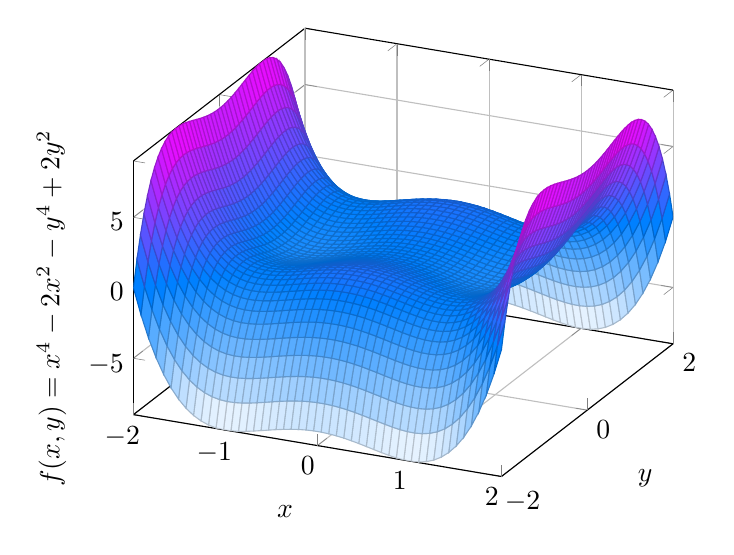
\begin{tikzpicture}
			\begin{axis}[
					colormap/cool,
					grid=both,
					domain=-2:2,
					domain y=-2:2,
					enlargelimits=false,
					xlabel=$x$,
					ylabel=$y$,
					zlabel={$f(x,y) = x^4 - 2x^2 - y^4 + 2y^2$},
					samples=50,
					z buffer=sort
				]
				\addplot3[surf] {x^4 - 2*x^2 - y^4 + 2*y^2};
			\end{axis}
		\end{tikzpicture}
	\end{center}

	The partial derivative of a function \( f(x, y) \) with respect to \( x \) at a point \( P = (x_0, y_0) \) is defined as:

	\[
		f_x(x_0, y_0) = \lim_{h \to 0} \frac{f(x_0 + h, y_0) - f(x_0, y_0)}{h}
	\]

	Similarly, the partial derivative with respect to \( y \) at \( P = (x_0, y_0) \) is:

	\[
		f_y(x_0, y_0) = \lim_{k \to 0} \frac{f(x_0, y_0 + k) - f(x_0, y_0)}{k}
	\]

	For the function \( f(x, y) = x^4 - 2x^2 - y^4 + 2y^2 \), the partial derivatives are:

	\[
		f_x(x, y) = 4x^3 - 4x, \quad f_y(x, y) = -4y^3 + 4y
	\]

}

\subsection{Differentiability}

\thm{Conditions for Differentiability}{Consider a function $f(x, y)$, and we aim to analyze the differentiability at a point $(a, b)$.

	To say that $f(x, y)$ is differentiable at the point $(a, b)$, the following conditions must hold:

	\begin{enumerate}
		\item The partial derivatives $f_x(a, b)$ and $f_y(a, b)$ must exist.
		\item We must have the following expression for the increment of $f$ at $(a, b)$:
		      \[
			      f(a + \Delta x, b + \Delta y) - f(a, b) = \Delta x f_x(a, b) + \Delta y f_y(a, b) + \epsilon_1(\Delta x) \Delta x + \epsilon_2(\Delta y) \Delta y
		      \]
		      where $\epsilon_1(\Delta x) \to 0$ as $\Delta x \to 0$ and $\epsilon_2(\Delta y) \to 0$ as $\Delta y \to 0$.
	\end{enumerate}

	This form shows that the change in the function can be approximated by the linear part involving the partial derivatives, with the higher-order terms represented by $\epsilon_1$ and $\epsilon_2$, which tend to zero.
}

\subsection*{Graphical Interpretation}

Consider the following illustration of the change in the function $f$:

\[
	\text{Elevation of } f(a, b) \to f(a + \Delta x, b + \Delta y)
\]

The increment of $f$ is given by:
\[
	f(a + \Delta x, b + \Delta y) - f(a, b)
\]

Using the definition of differentiability, we can decompose this increment as follows:

\[
	\Delta f = \Delta x f_x(a, b) + \Delta y f_y(a, b)
\]

Graphically, this can be interpreted as moving along the tangent plane at the point $(a, b)$ in the direction of $\Delta x$ and $\Delta y$. The elevation changes linearly based on the partial derivatives.

For the function to be differentiable at $(a, b)$, we require that:

\[
	\lim_{\Delta x \to 0} \epsilon_1(\Delta x) = 0, \quad \lim_{\Delta y \to 0} \epsilon_2(\Delta y) = 0
\]

These conditions ensure that the error terms involving $\epsilon_1$ and $\epsilon_2$ vanish as the changes $\Delta x$ and $\Delta y$ become small, ensuring a linear approximation near the point $(a, b)$.

\subsection{Open and Closed Sets}

Consider the set $R$ defined by:

\[
	R: y < x, \quad x^2 + y^2 < 1
\]

The set $R$ is open if we can draw it using **dashed lines**, indicating that the boundary is not included in the set. If we have a set of solutions to inequalities with strict inequalities (e.g., $<$ or $>$), the set is typically **open**.

If $R$ is defined by inequalities involving $\leq$ or $\geq$, then the set is **closed**.

\subsection*{Example of Open and Closed Sets}

Let $R_1$ be defined as:

\[
	R_1: x^2 + y^2 < 1 \quad \text{(open)}
\]

Let $S$ be defined as:

\[
	S: y < x \quad \text{(open)}
\]

We can also consider the closed sets:

\[
	R_2: x^2 + y^2 \leq 1 \quad \text{(closed)}
\]

\[
	S: y \leq x \quad \text{(closed)}
\]

Below are illustrations of open and closed sets. Dotted lines indicate that the boundary is **not included** (open), while solid lines indicate the boundary **is included** (closed).

\begin{center}
	\begin{tikzpicture}
		% Open set R: x^2 + y^2 < 1
		\draw[dashed] (0,0) circle (2);
		\node at (-2.5, 2.2) {$R_1$: $x^2 + y^2 < 1$};

		% Closed set R: x^2 + y^2 <= 1
		\draw (5,0) circle (2);
		\node at (8.5, 2.2) {$R_2$: $x^2 + y^2 \leq 1$};

		% Open set y < x
		\draw[dashed] (-3,-3) -- (3, 3);
		\node at (-3, 2.7) {Open $S: y < x$};

		% Closed set y <= x
		\draw (2, -3) -- (8, 3);
		\node at (8, 2.7) {Closed $S: y \leq x$};
	\end{tikzpicture}
\end{center}

\subsection{Conditions for Differentiability}

A function $f(x, y)$ is differentiable at $(a, b)$ if:

\begin{enumerate}
	\item The partial derivatives $f_x(a, b)$ and $f_y(a, b)$ exist.
	\item The following limit holds:
	      \[
		      f(a + \Delta x, b + \Delta y) - f(a, b) = \Delta x f_x(a, b) + \Delta y f_y(a, b) + \Delta x \epsilon_1(\Delta x) + \Delta y \epsilon_2(\Delta y)
	      \]
	      where $\epsilon_1(\Delta x) \to 0$ as $\Delta x \to 0$ and $\epsilon_2(\Delta y) \to 0$ as $\Delta y \to 0$.
\end{enumerate}

\thm{Sufficient Conditions for Differentiability}{

	A sufficient condition for differentiability is the following theorem:

	If there exists an open set $D$ containing $(a, b)$ such that $f_x(x, y)$ and $f_y(x, y)$ exist at all points in $D$, and if $f_x(a, b)$ and $f_y(a, b)$ are continuous at $(a, b)$, then $f(x, y)$ is differentiable at $(a, b)$.
}

\ex{Differentiability of a Given Function}{

	Consider the function:

	\[
		f(x, y) = e^{xy} + x^3 y
	\]

	We want to check whether this function is differentiable at any point $(a, b)$. First, we compute the partial derivatives:

	\[
		f_x(x, y) = y e^{xy} + 3x^2 y
	\]
	\[
		f_y(x, y) = x e^{xy} + x^3
	\]

	For any point $(a, b)$, both $f_x(a, b)$ and $f_y(a, b)$ exist in $\mathbb{R}^2$ and are continuous at $(a, b)$ because the terms $e^{xy}$, $x^3$, and $y$ are all continuous on $\mathbb{R}^2$.

	Thus, according to the theorem for differentiability, we conclude that:

	\[
		f(x, y) \text{ is differentiable at } (a, b)
	\]
}

\ex{Discontinuity of a Function}{

Consider the function:

\[
f(x, y) = 
\begin{cases}
    \frac{3xy}{x^2 + y^2} & \text{if } (x, y) \neq (0, 0) \\
    0 & \text{if } (x, y) = (0, 0)
\end{cases}
\]

We are interested in determining whether this function is continuous and differentiable at the point $(0, 0)$.

\subsection*{Continuity Check}

We first evaluate $f(0, 0)$:

\[
f(0, 0) = 0
\]

Next, we compute the limit of $f(x, y)$ as $(x, y) \to (0, 0)$. To do this, we examine the limit along two different paths:

\[
r_1(t) = \langle t, 0 \rangle
\]
Along this path, we have:

\[
\lim_{t \to 0} f(t, 0) = \lim_{t \to 0} \frac{3t \cdot 0}{t^2 + 0^2} = 0
\]

Now consider the path:

\[
r_2(t) = \langle t, t \rangle
\]
Along this path, we compute:

\[
\lim_{t \to 0} f(t, t) = \lim_{t \to 0} \frac{3t \cdot t}{t^2 + t^2} = \frac{3t^2}{2t^2} = \frac{3}{2}
\]

Since the limits along different paths do not agree (one is $0$, and the other is $\frac{3}{2}$), we conclude that:

\[
f(x, y) \text{ is not continuous at } (0, 0)
\]

Thus, even though the partial derivatives $f_x$ and $f_y$ exist at $(0, 0)$, the function is not continuous, and therefore, $f(x, y)$ is not differentiable at $(0, 0)$.
}

\begin{center}
    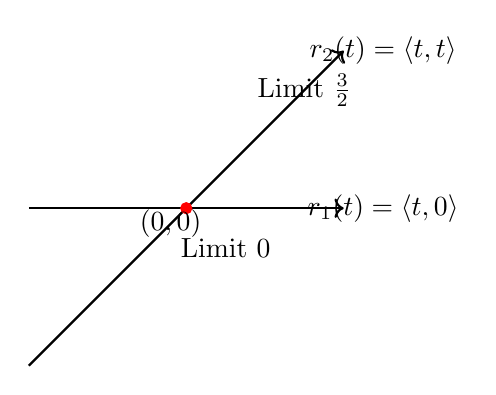
\begin{tikzpicture}
        % Path r_1: along x-axis
        \draw[->, thick] (-2,0) -- (2,0);
        \node at (2.5, 0) {$r_1(t) = \langle t, 0 \rangle$};

        % Path r_2: diagonal line
        \draw[->, thick] (-2,-2) -- (2,2);
        \node at (2.5, 2) {$r_2(t) = \langle t, t \rangle$};

        % Mark origin
        \filldraw[red] (0, 0) circle (2pt);
        \node at (-0.2, -0.2) {$(0,0)$};

        % Labels
        \node at (0.5, -0.5) {Limit $0$};
        \node at (1.5, 1.5) {Limit $\frac{3}{2}$};
    \end{tikzpicture}
\end{center}

\thm{Differentiability Implies Continuity}{

If $f(x, y)$ is differentiable at $(a, b)$, then $f(x, y)$ is also continuous at $(a, b)$. This is an important result that will help us analyze the next example.

}


\section{Directional Derivative}

Let $\mathbf{u} = \langle u_1, u_2 \rangle$ be a unit vector, i.e., $|\mathbf{u}| = 1$. The directional derivative of $f(x, y)$ at the point $(a, b)$ in the direction of $\mathbf{u}$ is defined as:

\[
	D_{\mathbf{u}} f(a, b) = \lim_{h \to 0} \frac{f(a + h u_1, b + h u_2) - f(a, b)}{h}
\]

This represents the slope of the hill that you are traveling on in the direction of $\mathbf{u}$.

If $f(x, y)$ is differentiable at $(a, b)$, we know that the function $f$ satisfies the following approximation:

\[
	f(a + \Delta x, b + \Delta y) - f(a, b) = \Delta x f_x(a, b) + \Delta y f_y(a, b) + \Delta x \epsilon_1(\Delta x) + \Delta y \epsilon_2(\Delta y)
\]

where $\epsilon_1(\Delta x) \to 0$ as $\Delta x \to 0$ and $\epsilon_2(\Delta y) \to 0$ as $\Delta y \to 0$.

\subsection{Derivation of the Directional Derivative}

Substituting $\Delta x = h u_1$ and $\Delta y = h u_2$, the directional derivative becomes:

\[
	\lim_{h \to 0} \frac{h u_1 f_x(a, b) + h u_2 f_y(a, b) + h u_1 \epsilon_1(h) + h u_2 \epsilon_2(h)}{h}
\]

Simplifying the expression:

\[
	= u_1 f_x(a, b) + u_2 f_y(a, b) + u_1 \epsilon_1(h) + u_2 \epsilon_2(h)
\]

As $h \to 0$, the terms $u_1 \epsilon_1(h)$ and $u_2 \epsilon_2(h)$ tend to $0$, so we are left with:

\[
	D_{\mathbf{u}} f(a, b) = u_1 f_x(a, b) + u_2 f_y(a, b)
\]

This can be expressed compactly as the dot product:

\[
	D_{\mathbf{u}} f(a, b) = \langle f_x(a, b), f_y(a, b) \rangle \cdot \mathbf{u}
\]

\dfn{Definition of the Gradient}{
	The gradient of $f(x, y)$ at the point $(a, b)$ is defined as the vector:

	\[
		\nabla f(a, b) = \langle f_x(a, b), f_y(a, b) \rangle
	\]

	The directional derivative is then the dot product of the gradient and the direction vector $\mathbf{u}$:

	\[
		D_{\mathbf{u}} f(a, b) = \nabla f(a, b) \cdot \mathbf{u}
	\]

	Thus, the gradient gives the direction of the steepest ascent of the function, and the directional derivative gives the rate of change of the function in the direction of $\mathbf{u}$.

}


\section{Application of the Gradient}

The gradient $\nabla f(a, b)$ plays an important role in determining the behavior of the function in various directions.

\subsection{Directional Derivative and the Gradient}

If $f$ is differentiable at $(a, b)$, then for any unit vector $\mathbf{u}$, the directional derivative of $f$ in the direction of $\mathbf{u}$ is given by:

\[
	D_{\mathbf{u}} f(a, b) = \nabla f(a, b) \cdot \mathbf{u}
\]

This formula can be used to determine how the function changes as we move in the direction of $\mathbf{u}$.

\subsection{Dot Product and Angle}

We know from vector calculus that:

\[
	\mathbf{u} \cdot \mathbf{v} = |\mathbf{u}| |\mathbf{v}| \cos \theta
\]

Thus, for the directional derivative:

\[
	D_{\mathbf{u}} f(a, b) = |\nabla f(a, b)| |\mathbf{u}| \cos \theta
\]

where $\theta$ is the angle between the gradient vector $\nabla f(a, b)$ and the direction vector $\mathbf{u}$.

\begin{itemize}
	\item If $\theta > \frac{\pi}{2}$, then $\mathbf{u}$ points downhill (negative directional derivative).
	\item If $0 < \theta < \frac{\pi}{2}$, then $\mathbf{u}$ points uphill (positive directional derivative).
\end{itemize}

\subsection{Maximum and Minimum Values of the Directional Derivative}

The directional derivative $D_{\mathbf{u}} f(a, b)$ is maximized when $\theta = 0^\circ$, which means that $\mathbf{u}$ points in the direction of the steepest ascent. This happens when $\mathbf{u}$ is in the same direction as $\nabla f(a, b)$:

\[
	\nabla f(a, b) \text{ points towards the direction of steepest ascent.}
\]

Conversely, the directional derivative is minimized when $\theta = 180^\circ$, which means $\mathbf{u}$ points in the direction of steepest descent. In this case:

\[
	-\nabla f(a, b) \text{ points towards the direction of steepest descent.}
\]

This forms the foundation of gradient descent algorithms, where the negative gradient is used to find minimum values.

\subsection{Tangent to a Level Curve}

Consider a level curve of the form $f(x, y) = c$. The vector $\nabla f(a, b)$ is perpendicular to the level curve at the point $(a, b)$, which implies that any vector $\mathbf{u}$ tangent to the level curve satisfies:

\[
	D_{\mathbf{u}} f(a, b) = 0
\]

This means that if $\mathbf{u}$ is tangent to the level curve, the directional derivative is zero, implying that there is no change in the value of the function along that curve.

Below is a diagram representing the gradient and the tangents to the level curves:

\begin{center}
	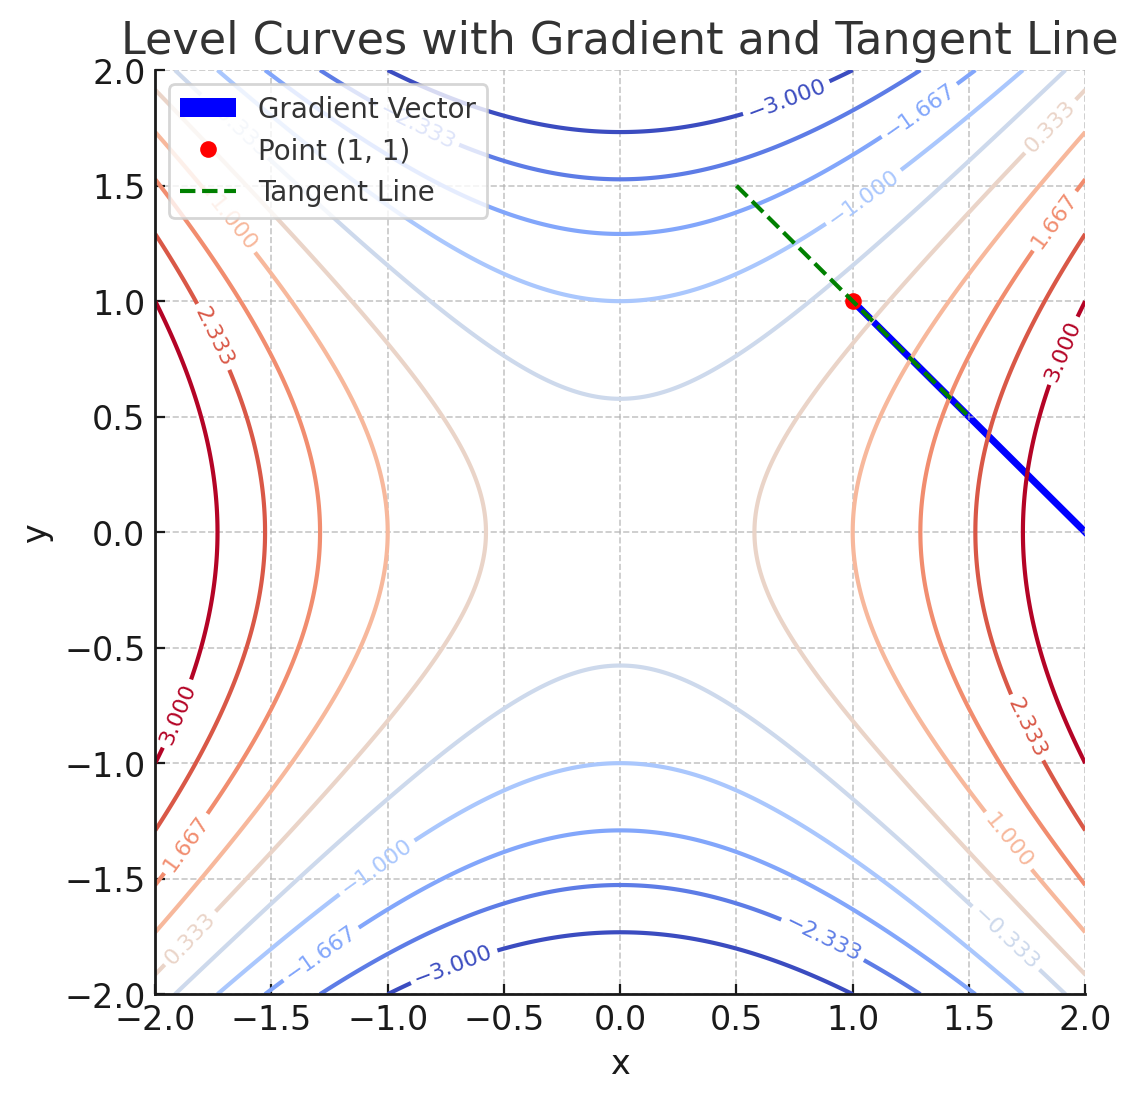
\includegraphics[scale=0.5]{levelcurves.png}
\end{center}

\section*{Tangent Planes}

The equation of the tangent plane to the surface $z = f(x, y)$ at the point $(a, b)$ is given by the linear approximation:

\[
	z = f(a, b) + \nabla f(a, b) \cdot \langle x - a, y - b \rangle
\]

This can be interpreted as the plane that best approximates the surface near the point $(a, b)$.

\subsection{Linear Approximation of Tangent Planes}

Using the gradient, we express the tangent plane as:

\[
	z = f(a, b) + f_x(a, b)(x - a) + f_y(a, b)(y - b)
\]

This equation is derived from the fact that the gradient $\nabla f(a, b) = \langle f_x(a, b), f_y(a, b) \rangle$ points in the direction of the steepest ascent.

Below is a simple diagram representing a surface and its tangent plane at a point:

\begin{center}
	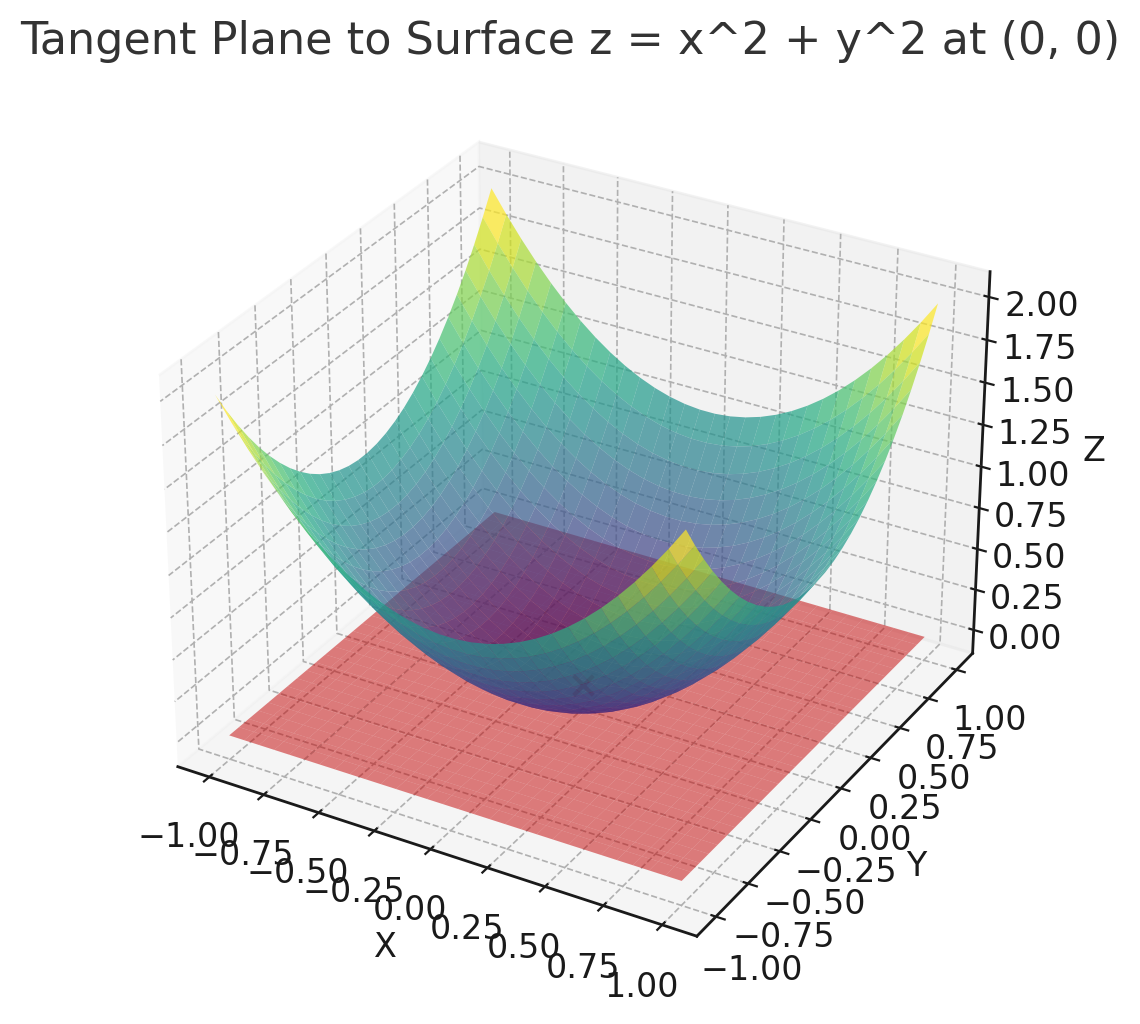
\includegraphics[scale=0.5]{tangentplane.png}
\end{center}


\end{document}